\section{Contexto histórico de la teoría de la coherencia}

	En el fondo, la coherencia plantea una única pregunta, casi infantil: ¿cuánto se parece una cosa a otra, y sobrevive ese parecido con el paso del tiempo? Suena demasiado simple para importar, y sin embargo la búsqueda de una respuesta rigurosa a esa pregunta creció, a lo largo de tres siglos, hasta convertirse en una de las grandes ideas unificadoras de la física: un lenguaje que explica por qué algunas fuentes de luz producen franjas de interferencia nítidas mientras que otras no producen ninguna, por qué un haz láser se comporta de forma tan distinta a la llama de una vela, cómo los radioastrónomos fotografían la sombra de un agujero negro sin construir jamás un telescopio del tamaño de la Tierra, y por qué las delicadas superposiciones dentro de un computador cuántico son tan exasperantemente difíciles de mantener con vida. La historia de la coherencia es en realidad dos historias que crecieron por separado y solo más tarde descubrieron que hablaban de lo mismo: una comienza en una mesa de apuestas en la Francia del siglo XVII, y la otra comienza en un laboratorio de óptica a oscuras. Vale la pena seguir ambos hilos desde el principio.

	El primer hilo es la historia de la correlación, y comienza, apropiadamente, con una apuesta. En 1654 el noble y jugador Antoine Gombaud, más conocido como el Chevalier de Méré, escribió a Blaise Pascal preguntando cómo debían repartirse justamente las apuestas de una partida de dados interrumpida entre dos jugadores. La correspondencia resultante entre Pascal y Pierre de Fermat, en la que resolvieron la matemática de la esperanza y la combinatoria necesarias para responder tales preguntas, se considera generalmente el nacimiento de la teoría de la probabilidad. Sus ideas maduraron lentamente. En 1713, sesenta años más tarde, el libro póstumo de Jacob Bernoulli, \textit{Ars Conjectandi} \cite{bernoulli1713}, demostró la ley de los grandes números, el notable hecho de que si se repite un experimento aleatorio suficientes veces, la frecuencia observada de un resultado se estabiliza, cada vez con más fiabilidad, en torno a su probabilidad teórica verdadera. Un siglo más tarde todavía, en 1812, Pierre Simon Laplace reunió estos resultados dispersos, junto con su propia teoría de cómo debe actualizarse nuestra creencia ante nueva evidencia (lo que hoy llamamos inferencia bayesiana), en la monumental \textit{Théorie Analytique des Probabilités} \cite{laplace1812theorie}. Lo que aún faltaba en toda esta tradición era un número, una única cifra capaz de decir no solo cuán incierta es una cantidad, sino cuán fuertemente se mueven juntas dos cantidades distintas.

	Ese número faltante llegó por una vía inesperada: el muy práctico oficio de tratar con mediciones ruidosas. En 1809, tratando de ajustar las observaciones imperfectas y dispersas de las órbitas planetarias, Carl Friedrich Gauss introdujo el método de mínimos cuadrados en su \textit{Theoria Motus} \cite{gauss1809theoria}, una técnica construida enteramente sobre la idea de que los errores se agrupan estadísticamente en torno a la verdad. Décadas más tarde, en la década de 1880, el polímata Francis Galton, fascinado por cuán fuertemente la estatura de un hijo tiende a seguir la de sus padres, acuñó la palabra misma ``correlación'' para describir precisamente este tipo de tendencia conjunta \cite{galton1888correlations}. Le correspondió a su alumno Karl Pearson, en 1896, convertir la intuición de Galton en una fórmula precisa: el coeficiente de correlación de Pearson \cite{pearson1896regression}, un único número, siempre entre menos uno y más uno, que indica de un vistazo si dos cantidades marchan juntas, se separan, o se ignoran por completo. Por primera vez, el parecido entre dos cosas podía medirse en lugar de simplemente percibirse.

	El segundo hilo, mientras tanto, se desarrollaba casi por completo sin referencia al primero, en el estudio de la luz misma. En 1801, Thomas Young dejó caer luz solar a través de dos rendijas estrechas y la vio pintar una hilera de bandas claras y oscuras en una pantalla detrás de ellas \cite{young1804bakerian}, la firma inconfundible de dos ondas que a veces se refuerzan y a veces se cancelan mutuamente. Para que esas franjas aparecieran, la luz que salía de las dos rendijas tenía que mantener una relación de fase estable y confiable consigo misma, una propiedad para la que nadie tenía todavía un nombre, aunque todos podían ver su huella en la pantalla. Entre 1815 y 1820, Augustin Jean Fresnel construyó la teoría matemática completa de la luz como onda transversal, y con ella la interferencia y la polarización dejaron de ser curiosidades para convertirse en consecuencias de una única imagen física. Y sin embargo un misterio persistía silenciosamente. El haz de Young, recién dividido a partir de una sola rendija estrecha, producía franjas hermosamente. Pero la luz de día ordinaria, o la luz de una vela, o la del Sol mismo, jamás producían nada semejante cuando simplemente se les dejaba interferir con una copia retardada de sí mismas más allá de cierta separación. Algo en la luz real y cotidiana era distinto de la onda idealizada y perfectamente regular que describía la matemática de Fresnel, y durante cien años nadie pudo decir exactamente qué.

	La respuesta, cuando finalmente llegó en el siglo XX, es que las fuentes de luz ordinarias no son en absoluto ondas únicas y ordenadas. Un filamento caliente, una llama, o la superficie del Sol es una enorme multitud de átomos independientes, cada uno emitiendo su propio destello breve de luz y luego callando, completamente desacompasado de sus vecinos, de modo que la onda global forma y reforma su fase miles de millones de veces por segundo de una manera que, a todos los efectos prácticos, es aleatoria. Describir correctamente semejante luz significaba casar las dos tradiciones separadas que habían crecido de forma aislada: la maquinaria estadística de Pascal, Gauss, Galton y Pearson debía injertarse en la óptica ondulatoria de Young y Fresnel. Ese injerto es exactamente lo que la palabra ``coherencia'' designa hoy: no si una onda tiene una fase, toda onda la tiene, sino si esa fase permanece suficientemente predecible, durante suficiente tiempo y sobre una región suficientemente amplia, como para dejar un rastro visible cuando se hace que la onda interfiera con una copia de sí misma.

	El paso matemático decisivo se dio en la década de 1930. En 1934 el físico neerlandés Pieter Hendrik van Cittert resolvió cómo cambian las correlaciones estadísticas de la luz proveniente de una fuente incoherente y extendida, una estrella distante, por ejemplo, a medida que esa luz se aleja de la fuente \cite{vancittert1934}, y en 1938 Frits Zernike afinó y generalizó el resultado hasta el teorema que hoy lleva ambos nombres \cite{zernike1938}. El teorema de van Cittert-Zernike hace una afirmación hermosamente contraintuitiva: una luz que comienza siendo completamente incoherente, con cada punto de la fuente parpadeando independientemente de todos los demás, se vuelve medible y predeciblemente más coherente por el mero hecho de recorrer una gran distancia. Esto no es una nota al pie menor. Es el principio físico que permite a los astrónomos medir el tamaño angular de estrellas demasiado pequeñas para que cualquier telescopio las resuelva directamente, comparando la luz recogida en dos puntos separados y observando cómo se desvanecen las franjas a medida que crece la separación, exactamente el truco que Albert Michelson y Francis Pease usaron en 1920 para medir el diámetro de la gigante roja Betelgeuse \cite{michelson1921diameter}. Décadas después, ese mismo teorema, escalado de un puñado de metros a una red de antenas de radio que abarca todo el planeta, es lo que permitió a la colaboración del Telescopio del Horizonte de Sucesos reconstruir, en 2019, la primera imagen directa de un agujero negro.

	La teoría clásica de la coherencia encontró su forma definitiva y madura en el trabajo de Max Born y Emil Wolf, cuyo tratado \textit{Principles of Optics} \cite{born1999principles} reunió cada hebra en un solo objeto, la función de coherencia mutua, que simplemente mide cuán correlacionada está la onda luminosa entre dos puntos del espacio y dos instantes de tiempo. Comprimidas dentro de esa única función están las dos cualidades que de verdad interesan a un experimentador: la coherencia temporal, esencialmente cuán puro es el color de la luz y durante cuánto tiempo mantiene un ritmo estable consigo misma, y la coherencia espacial, cuán fielmente la onda se mantiene acompasada a lo largo de una región extendida en lugar de solo en un punto. Leonard Mandel y Wolf ampliaron más tarde esta imagen en el tratado completo \textit{Optical Coherence and Quantum Optics} \cite{mandel1995optical}, afinando las nociones prácticas de tiempo de coherencia y longitud de coherencia que hoy todo laboratorio da por sentadas. Nada de esto quedó confinado al tablero. El interferómetro de Michelson de la década de 1890 ya explotaba la coherencia temporal para medir longitudes de onda con una precisión que ninguna regla podía igualar, y la invención del láser en 1960, cuya luz es coherente en un grado que ninguna fuente natural alcanza jamás, convirtió la coherencia de un tema de fascinación teórica en el principio de funcionamiento detrás de las comunicaciones por fibra óptica, la metrología de precisión, la holografía y la medicina moderna.

	Tampoco la coherencia pertenece solo a la óptica. Dondequiera que muchas partes independientes de un sistema puedan hacerse oscilar al unísono, aparece algo con exactamente la misma anatomía matemática. En física de la materia condensada, la superconductividad es, en el fondo, un fenómeno de coherencia: por debajo de una temperatura crítica, una enorme población de electrones apareados se bloquea en una única fase cuántica compartida a través de toda una muestra macroscópica, razón por la cual una supercorriente fluye sin resistencia alguna. La resonancia magnética nuclear y la resonancia magnética de imágenes construida sobre ella funcionan inclinando miles de millones de espines nucleares hacia una precesión común y coherente, y observando luego, con exquisita sensibilidad, cuán rápido decae ese ritmo compartido. Todo reloj atómico, y con él el sistema de posicionamiento global entero, depende de un oscilador cuya fase permanece coherente durante todo el tiempo humanamente alcanzable. La coherencia, en resumen, no es una peculiaridad de la luz; es lo que permite que innumerables actores independientes, electrones, espines, átomos o fotones, se comporten, brevemente y con fragilidad, como uno solo.

	Mientras toda esta maquinaria clásica se consolidaba, una historia completamente distinta y más extraña se desarrollaba en el mundo cuántico. Su escena inicial tuvo lugar en 1956, cuando Robert Hanbury Brown y Richard Twiss, tratando de medir los tamaños angulares de las estrellas con detectores de radio y luego ópticos, descubrieron que los fotones que llegaban de una fuente térmica a dos detectores separados no eran independientes: tendían a llegar en pequeños grupos correlacionados \cite{hanburybrown1956correlation}. El resultado parecía a muchos físicos de la época sencillamente imposible. Los fotones, se suponía, debían comportarse como partículas clásicas e independientes una vez detectados, y ninguna correlación semejante debía sobrevivir al acto de la medición; siguió una controversia real y animada antes de que el efecto fuera aceptado. Desenredarlo correctamente requería una teoría plenamente cuántica de la coherencia, y esa teoría fue provista en 1963, casi simultánea e independientemente, por Roy Glauber \cite{glauber1963quantum} y George Sudarshan \cite{sudarshan1963equivalence}. Glauber introdujo los estados coherentes, los estados cuánticos de la luz que se comportan tan cerca como la mecánica cuántica lo permite de las ondas clásicas de Fresnel, y definió toda una jerarquía de funciones de correlación cuánticas capaces de explicar rigurosamente el agrupamiento de Hanbury Brown y Twiss, y de predecir su imagen especular, el antiagrupamiento de fotones, un comportamiento tan tercamente no clásico que ninguna teoría ondulatoria de la luz podría jamás reproducirlo, confirmado más tarde en el laboratorio. Sudarshan, trabajando desde una dirección distinta, encontró la frontera matemática precisa, hoy llamada representación de Glauber-Sudarshan, que separa la luz cuya naturaleza cuántica puede ignorarse con seguridad de aquella para la cual no puede. Por esta teoría cuántica de la coherencia óptica, Glauber recibió el Premio Nobel en 2005, y el campo que fundó es lo que hoy llamamos óptica cuántica.

	La coherencia cuántica resultó importar por razones que van mucho más allá del conteo de fotones. Es la coherencia cuántica, la delicada superposición de fase fija de muchos estados posibles a la vez, lo que hace que un bit cuántico sea fundamentalmente distinto de uno ordinario, y es la pérdida de esa coherencia por el contacto inevitable con el entorno, un proceso que los físicos llaman decoherencia, lo que explica por qué el mundo cotidiano a nuestro alrededor luce tan tercamente clásico aunque esté construido a partir de partes cuánticas. Mantener la coherencia con vida el tiempo suficiente para que sea útil es, hasta el día de hoy, el mayor obstáculo de ingeniería que se interpone entre los computadores cuánticos de hoy y los del mañana. La misma idea reaparece en la materia más fría que los físicos saben producir: en 1995 Eric Cornell, Carl Wieman y Wolfgang Ketterle enfriaron nubes de átomos a temperaturas de nanokelvin y observaron a millones de ellos colapsar en un único estado cuántico compartido, un condensado de Bose-Einstein, en efecto una enorme onda de materia coherente, un logro reconocido con el Premio Nobel en 2001. Incluso alcanza a la biología: experimentos cuidadosos sobre los complejos captadores de luz que las plantas y ciertas bacterias usan para capturar la luz solar han encontrado que la coherencia cuántica en la transferencia de esa energía sobrevive, asombrosamente, durante fracciones medibles de segundo a temperatura ambiente, sugiriendo que la evolución pudo haber tropezado con la coherencia cuántica y explotado mucho antes de que los físicos le dieran un nombre.

	Uniendo las imágenes estadística y ondulatoria de la coherencia, tanto clásica como cuántica, hay una única pieza de matemática: el teorema de Wiener-Khinchin, desarrollado independientemente por Norbert Wiener en 1930 \cite{wiener1930generalized} y Aleksandr Khinchin en 1934 \cite{khinchin1934korrelationstheorie}, que establece que la correlación de una señal fluctuante consigo misma y la manera en que la energía de esa señal se distribuye en frecuencia son simplemente dos caras del mismo objeto, traducidas la una a la otra mediante una transformada de Fourier. Es, como mostrarán los capítulos posteriores, la bisagra matemática silenciosa sobre la que gira todo el tema.

	En el siglo XXI la coherencia ha adquirido una identidad más: hoy se entiende, y se cuantifica formalmente, como un recurso físico genuino, algo que puede crearse, gastarse y agotarse casi como la energía o el entrelazamiento, con sus propias reglas de contabilidad rigurosas dentro de la teoría más amplia de la información cuántica \cite{baumgratz2014quantifying}. Vista de principio a fin, la historia de la coherencia recorre desde un argumento del siglo XVII sobre dados, pasando por la estadística de la estatura heredada y la interferencia de la luz solar, hasta la formación de imágenes de un agujero negro y el frágil funcionamiento interno de un procesador cuántico. En su forma clásica explica por qué las estrellas titilan como lo hacen, por qué un láser puede cortar acero mientras que una antorcha no puede, y por qué un interferómetro del tamaño de un planeta puede fotografiar algo que ningún telescopio individual pudo jamás. En su forma cuántica explica por qué el mundo de los átomos se siente tan distinto del mundo de las mesas y las sillas, y hoy se sitúa en el centro mismo del esfuerzo por construir tecnologías que piensen y se comuniquen de maneras que ninguna máquina clásica pudo jamás. La coherencia, ya se cuente en tiradas de dados correlacionadas, ondas de luz que interfieren o qubits entrelazados, es en último término siempre lo mismo: el orden, sobreviviendo breve y notablemente en un mundo que constantemente conspira para borrarlo.

\section{¿Cómo se cuantifica la similaridad estadística?}

	Supongamos que tenemos un fenómeno completamente aleatorio, como la radiación electromagnética emitida por una bombilla incandescente que no está en equilibrio termodinámico, el número de automóviles en alguna ciudad capital a lo largo del día, el movimiento de un ion en un plasma, o algo tan simple como lanzar una pelota al aire en condiciones no ideales.

	Cuando deseamos analizar estadísticamente un único objeto o variable aleatoria, aparecen las herramientas familiares: la densidad de probabilidad, el valor medio, la desviación estándar, la curtosis, etcétera. ¿Qué ocurre cuando queremos estudiar al menos dos variables aleatorias y cómo se relacionan? Cuando deseamos estudiar la estadística de dos o más variables aleatorias debemos estudiar la similaridad estadística entre ellas; pero la similaridad estadística es un concepto bastante amplio, pues podemos tener similaridad en los valores medios, o en las desviaciones estándar, o en las densidades de probabilidad. Para abordar este problema volvemos al álgebra lineal.

	Si tenemos dos vectores $\vec{A},\vec{B} \in \mathbb{R}^n$, el producto punto $\vec{A}\cdot\vec{B}$ se interpreta como la magnitud de la proyección de $\vec{A}$ sobre $\vec{B}$ y viceversa; también puede leerse como \textit{cuánto de $\vec{A}$ yace a lo largo de $\vec{B}$}.

	Vale la pena detenerse en lo que esa operación en verdad hace mecánicamente, porque toda la teoría de la coherencia está construida sobre este único gesto. Escrito componente a componente, el producto punto es
	\begin{equation}\label{eq:DotComponents}
		\vec{A}\cdot\vec{B} = \sum_{i=1}^{n} A_i B_i,
	\end{equation}
	es decir, \textit{multiplíquense las dos listas entrada por entrada y súmense los resultados}. Nada más. Y sin embargo el signo de cada término individual ya lleva exactamente la información que buscamos: siempre que $A_i$ y $B_i$ se inclinan hacia el mismo lado, su producto es positivo y empuja la suma hacia arriba; siempre que se inclinan hacia lados opuestos, el producto es negativo y la arrastra hacia abajo. Si los dos vectores tienden a coincidir a lo largo de la mayoría de sus componentes, los términos positivos dominan y el total resulta grande; si sistemáticamente discrepan, el total resulta grande pero negativo; y si coinciden con la misma frecuencia con que discrepan, los términos se cancelan mutuamente en la suma y el total colapsa a casi cero. Así, ``multiplicar los pares y sumar'' es ya, por sí solo, un medidor de similaridad, y todo lo que sigue en este capítulo es ese mismo gesto aplicado a objetos progresivamente más ricos.

	Este comportamiento puede extrapolarse a espacios vectoriales continuos, donde suele emplearse la noción de producto interno. El paso es más pequeño de lo que parece: una función es simplemente un vector con un continuo de componentes, pues en lugar de la lista finita $A_1,A_2,\dots,A_n$ ahora llevamos los valores $f_A(x)$, uno para cada $x$. El índice $i$ se convierte en la etiqueta $x$, la suma sobre un índice discreto se convierte en una integral sobre uno continuo, y el producto punto se convierte en el producto interno. Si $f_A , f_B$ son dos elementos del espacio de Hilbert $L^2(\mathbb{R})$ de funciones de cuadrado integrable de una variable real, puede definirse un producto interno como

	\begin{equation}\label{eq:ProdIn}
		\braket{f_A,f_B} = \int_\mathbb{R} f_A^*(x)f_B(x) W(x)\,dx,
	\end{equation}

	donde el conjugado complejo en el primer factor es lo que mantiene a $\braket{f_A,f_A}$ real y no negativo incluso cuando las funciones son complejas, como lo serán los campos ópticos de este capítulo, y donde $W(x)$ es alguna función de peso.\footnote{$W(x)$ recibe este nombre porque, como su nombre indica, otorga un peso a cada valor que el integrando pueda tomar; no hay contribuciones uniformes, sino que cada valor posible del integrando dentro del dominio contribuye ponderado por el valor de $W$ en ese punto.} La interpretación sigue siendo válida: esto puede leerse como cuánto coincide la función $f_A$ sobre todos los reales con la función $f_B$ sobre todos los reales.

	Para llegar a la noción de correlación a partir del álgebra lineal usamos un poco de notación bra-ket, donde el ket $\ket{f_A}$ representa un vector de un espacio de Hilbert $L^2$ arbitrario y el bra $\bra{f_A}$ representa un elemento del dual del mismo espacio de Hilbert,\footnote{El espacio de Hilbert es un caso particular de los espacios $L^p$, el espacio de funcionales Lebesgue-integrables de norma $p$; para Hilbert $p=2$, y tiene la propiedad de que el dual de $L^2$ es también $L^2$, lo que permite que la mecánica cuántica surja naturalmente en este espacio.} y el producto interno de un estado consigo mismo, $\braket{f_A,f_A}= \braket{f_A|f_A}$, acumula la probabilidad de encontrar el sistema en cualquier lugar; es el integrando $|f_A(q)|^2$, más que la integral completada, el que juega el papel de la densidad de probabilidad de encontrar $f_A$ en un estado $q \pm \triangle q$, donde $q$ representa alguna coordenada generalizada. Supongamos que $f_A,f_B \in L^2$ tienen la forma

	\begin{equation}
		\ket{f_A} = \hat{A}\ket{\Psi_A}, \quad \ket{f_B} = \hat{B}\ket{\Psi_B},
	\end{equation}

	donde $\hat{A},\hat{B}$ son los operadores de las magnitudes físicas de $\ket{\Psi_A},\ket{\Psi_B}$, de modo que podemos interpretar $\ket{f_A},\ket{f_B}$ como las funciones de onda gobernadas por su valor esperado. Usando el producto interno \eqref{eq:ProdIn} con función de peso unitaria, $W=1$, el producto interno se lee

	\begin{equation}
		\braket{f_A | f_B} = \int_{\mathbb{R}^n} \hat{A}\hat{B} \braket{\Psi_A|\Psi_B}\, d^nq = \int_{\mathbb{R}^n} \hat{A}\hat{B}\, P(A;B)\, d^nq,
	\end{equation}

	donde vemos que la similaridad entre $\ket{f_A}$ y $\ket{f_B}$ puede verse como el producto de $\hat{A}$ con $\hat{B}$ multiplicado por la densidad de probabilidad de tener los estados $A$ y $B$.\footnote{Este último paso es deliberadamente heurístico: estamos tratando los operadores como si pudieran simplemente sacarse del producto interno y reemplazarse por los valores que miden, lo cual solo es legítimo cuando actúan sobre sus propios autoestados. El propósito aquí no es una derivación sino un puente, para hacer plausible de dónde viene la definición que sigue; el tratamiento riguroso pertenece a \cite{mandel1995optical}.} Es decir, la similaridad, o cuán \textit{correlacionadas} están dos variables, puede verse como la integral del producto de las variables multiplicada por su densidad de probabilidad conjunta.

	Con esta analogía en mente podemos entender la correlación como una primera medida de la similaridad entre una o más variables a través del espacio y del tiempo. Si $x_1(\vec{r},t_1), x_2(\vec{r}',t_2)$ son dos variables aleatorias y $p_2(x_1,t_1;x_2,t_2)$ es la densidad de probabilidad conjunta, entonces la correlación entre $x_1,x_2$ se define como

	\begin{equation}\label{eq:CorrFunc}
		\Gamma(\vec{r},\vec{r}';t_1,t_2) = E\left\{ x_1(\vec{r},t_1) x_2^*(\vec{r}',t_2)\right\}
		= \int\!\!\int x_1 x_2^* \; p_2(x_1,t_1;x_2,t_2)\, dx_1 dx_2,
	\end{equation}

	es decir, como el promedio de ensamble de $x_1\cdot x_2^*$, ponderado por cuán probable es que cada par de valores ocurra conjuntamente. La conjugación se coloca aquí en el segundo factor para concordar con la convención usada para la función de coherencia en la siguiente sección; para variables reales no hace nada en absoluto, y para las complejas simplemente conjuga a $\Gamma$ en su totalidad, sin afectar ninguna magnitud que nos vaya a interesar.

	Estructuralmente este es el mismo objeto que hemos venido construyendo todo este tiempo. La suma sobre componentes en \eqref{eq:DotComponents} se ha convertido simplemente en un promedio sobre el ensamble, y el papel de la función de peso $W$ en \eqref{eq:ProdIn} lo desempeña ahora la densidad de probabilidad conjunta $p_2$, que es el peso natural a usar cuando las ``componentes'' que se emparejan son los resultados posibles de un experimento aleatorio en lugar de las entradas de una lista. La correlación, en otras palabras, es el producto punto de dos variables aleatorias, tomado en el único sentido disponible cuando las cantidades involucradas se niegan a quedarse quietas.

	El mismo argumento del signo que convirtió al producto punto en un medidor de similaridad nos dice ahora cómo leer $\Gamma$, y vale la pena exponer los tres casos explícitamente. Si las dos variables suben y bajan juntas, de modo que son grandes en los mismos instantes y pequeñas en los mismos instantes, entonces el producto $x_1 x_2^*$ es predominantemente positivo, cada realización del experimento contribuye con el mismo signo, y el promedio sobrevive como un número positivo grande. Si se mueven en oposición estricta, una alcanzando su pico cada vez que la otra alcanza su valle, el producto es predominantemente negativo y el promedio sobrevive como un número negativo grande, lo cual es igualmente informativo: la anticorrelación perfecta es una forma de similaridad perfecta, simplemente con un signo adjunto. Pero si las dos variables no saben nada la una de la otra, entonces por cada realización en la que el producto resulta ser positivo hay, en algún lugar del ensamble, una realización igualmente probable en la que resulta negativo, las contribuciones se aniquilan mutuamente, y el promedio colapsa a cero. \textbf{El promediado no es, por tanto, un tecnicismo incidental sino el mecanismo entero}: es precisamente lo que destruye los términos que no llevan información compartida mientras permite que los términos que sí la llevan se acumulen.

	Dos rasgos de la definición \eqref{eq:CorrFunc} merecen un comentario, porque ambos difieren del coeficiente de Pearson visto en la introducción histórica. El primero es que no hemos restado los valores medios antes de multiplicar. Restarlos produciría la covarianza, que pregunta cómo conspiran las \textit{fluctuaciones} en torno al promedio; conservarlos, como hacemos aquí, pregunta por la cantidad total, y para los campos ópticos de este capítulo la distinción felizmente se desvanece, pues un campo térmico oscila simétricamente en torno a cero y su media se anula por sí sola. El segundo es que no hemos dividido por nada, de modo que $\Gamma$ todavía lleva las unidades físicas de los campos con los que fue construida y su magnitud depende de cuán intensa resulta ser la luz, no solo de cuán similar es. Una correlación de $10^{-6}$ entre dos haces débiles puede representar un acuerdo mucho más estrecho que una correlación de la unidad entre dos haces potentes. Reparar esto, dividiendo $\Gamma$ por su propio valor a separación nula, que es precisamente la intensidad, de modo que el resultado sea un número puro confinado entre cero y uno que mida similaridad y solo similaridad, es exactamente el paso que convierte a la función de correlación en el \textit{grado complejo de coherencia}, y es el punto hacia el que trabaja la siguiente sección.

\section{Variables aleatorias}\label{sec:RandomVariables}

	En la sección anterior hablamos libremente de variables aleatorias, de densidades de probabilidad conjuntas y de promedios de ensamble, y lo hicimos a propósito, porque el objetivo allí era hacer plausible la definición de la función de correlación, no justificarla. Esa deuda debe pagarse ahora. La teoría de la coherencia es, de principio a fin, una teoría \textit{sobre} promedios, y un promedio que no está definido con precisión no define nada con precisión. Peor aún, los objetos que manipularemos no son promedios de números sino promedios sobre una colección infinita de historias de campo enteras, y para tales objetos la intuición ingenua no es meramente imprecisa, sino que en ocasiones es sencillamente errónea.

	El propósito de esta sección es, por tanto, construir la noción de variable aleatoria desde los cimientos, en el lenguaje de la teoría de la medida en el que fue formulada por Kolmogórov \citep{kolmogorov1933grundbegriffe}, y luego aplicarla al campo electromagnético vectorial, construyendo explícitamente el espacio de probabilidad sobre el cual vive toda la teoría que sigue. Cada ingrediente recibirá su lectura física a medida que aparezca, porque cada uno de ellos corresponde a algo que un óptico hace en un laboratorio.

	\subsection{El espacio muestral y el significado físico de un evento}

		\begin{myDef}
			\textit{(Espacio muestral)} Un \textit{espacio muestral} es un conjunto no vacío $\Omega$. Sus elementos $\omega\in\Omega$ se llaman \textit{resultados elementales} o \textit{puntos muestrales}.
		\end{myDef}

		La tentación es leer $\omega$ como un número, y es esencial resistirla. En óptica un resultado elemental no es un valor de campo ni una medición; es una \textit{realización} completa de la fuente, es decir, una historia espaciotemporal entera que el campo podría haber tenido. Una lámpara térmica contiene del orden de $10^{20}$ átomos radiando independientemente, cada uno con un instante de emisión y una fase inicial que ni controlamos ni conocemos. Una asignación particular de todos esos detalles microscópicos, junto con todo lo que se sigue de ella mediante las ecuaciones de Maxwell, es un $\omega$. El conjunto de todas esas asignaciones es $\Omega$.

		Esta es precisamente la imagen que mostrará la Figura~\ref{fig:randomvar} en la sección siguiente, donde se dibujan varias curvas $^{(i)}E(\vec{r},t)$ una encima de otra: cada curva es un $\omega$, y la etiqueta $i$ es solo un recurso de contabilidad, pues en general $\Omega$ es no numerable. Lo que el laboratorio entrega en una tarde cualquiera es un único $\omega$, elegido por la naturaleza y no revelado a nosotros. La totalidad de la óptica estadística consiste en extraer afirmaciones sobre $\Omega$ a partir del acceso a uno solo de sus puntos.

		\begin{myDef}
			\textit{(Evento)} Un \textit{evento} es un subconjunto $A\subseteq\Omega$.
		\end{myDef}

		El contenido físico de esta definición es que un evento es un \textbf{enunciado sobre la realización que puede declararse verdadero o falso}. El enunciado ``el campo en $\vec{r}_{0}$ en el instante $t_{0}$ superó el valor $E_{0}$'' no es un número; es el conjunto de todas las realizaciones para las cuales ocurre que eso es el caso. Decir que el evento ocurrió es decir que el $\omega$ que la naturaleza seleccionó pertenece a ese subconjunto. Eventos y enunciados son la misma cosa vista desde dos lados, y esta identificación es lo que permite construir la probabilidad a partir de la teoría de conjuntos.

	\subsection{La sigma-álgebra, o qué preguntas pueden formularse}

		\begin{myDef}
			\textit{(Sigma-álgebra)} Una \textit{sigma-álgebra} sobre $\Omega$ es una colección $\mathcal{F}$ de subconjuntos de $\Omega$ tal que
			\begin{enumerate}
				\item $\Omega\in\mathcal{F}$,
				\item si $A\in\mathcal{F}$ entonces $A^{c} = \Omega\setminus A\in\mathcal{F}$,
				\item si $A_{1},A_{2},A_{3},\dots\in\mathcal{F}$ entonces $\bigcup_{n=1}^{\infty}A_{n}\in\mathcal{F}$.
			\end{enumerate}
			El par $(\Omega,\mathcal{F})$ se llama \textit{espacio medible}.
		\end{myDef}

		Una sigma-álgebra parece una pieza de contabilidad y es, de hecho, un enunciado físico. Es el \textit{catálogo de preguntas admisibles}, la lista de enunciados a los que la teoría está preparada para asignar una probabilidad, y los tres axiomas son exactamente las tres propiedades que cualquier catálogo honesto de preguntas debe tener.

		El primero dice que la pregunta ``¿ocurrió algo en absoluto?'' es admisible. El segundo dice que si podemos preguntar si un evento ocurrió, podemos preguntar si no ocurrió, lo cual es la expresión formal del hecho de que un aparato capaz de detectar algo es, por ese mismo hecho, capaz de detectar su ausencia. El tercero dice que si cada una de una sucesión de preguntas es admisible, también lo es la pregunta de si al menos una de ellas se cumple.

		La palabra \textit{numerable} en el tercer axioma no es una conveniencia técnica sino una restricción física genuina, y merece señalarse. Cualquier protocolo experimental real es una \textit{sucesión} de operaciones: se registra una lectura, luego otra, luego otra. Ningún laboratorio ha realizado jamás una cantidad no numerable de operaciones, y la teoría está construida para no prometer nada sobre lo que ocurriría si se pudiera.

		Cabría preguntarse por qué no tomamos simplemente $\mathcal{F}$ como la colección de \textit{todos} los subconjuntos de $\Omega$ y asunto terminado. La respuesta es que no se nos permite hacerlo. Vitali demostró en 1905 \citep{vitali1905problema} que en la recta real existen conjuntos tan patológicos que ninguna noción de tamaño invariante bajo traslación puede asignárseles sin contradicción. Si insistiéramos en medirlo todo nos veríamos forzados a la inconsistencia, y la sigma-álgebra es precisamente el dispositivo que mantiene semejantes monstruos fuera de la teoría mientras conserva todo conjunto sobre el que un físico tendría ocasión de preguntar alguna vez.

		El ejemplo que necesitaremos constantemente es el siguiente.

		\begin{myDef}
			\textit{(Sigma-álgebra de Borel)} La \textit{sigma-álgebra de Borel} $\mathcal{B}(\mathbb{R}^{n})$ es la sigma-álgebra más pequeña sobre $\mathbb{R}^{n}$ que contiene todos los conjuntos abiertos.
		\end{myDef}

		Físicamente, $\mathcal{B}(\mathbb{R})$ está generada por las preguntas ``¿la lectura está entre $a$ y $b$?'', junto con todo lo que puede construirse a partir de una cantidad numerable de tales preguntas mediante negación y unión. Esta es exactamente la clase de preguntas que un detector real, que tiene una resolución finita y reporta un intervalo en lugar de un punto, es capaz de responder. La sigma-álgebra de Borel no es una abstracción impuesta a la física; es la transcripción matemática de lo que hace un instrumento graduado.

	\subsection{Medida, la medida de Lebesgue y la medida de probabilidad}

		\begin{myDef}
			\textit{(Medida)} Una \textit{medida} sobre un espacio medible $(\Omega,\mathcal{F})$ es una función $\mu:\mathcal{F}\to[0,\infty]$ tal que $\mu(\emptyset)=0$ y tal que, para toda sucesión $A_{1},A_{2},\dots$ de elementos de $\mathcal{F}$ disjuntos dos a dos,
			\begin{equation}\label{eq:CountableAdditivity}
				\mu\left(\bigcup_{n=1}^{\infty}A_{n}\right) = \sum_{n=1}^{\infty}\mu(A_{n}).
			\end{equation}
			La terna $(\Omega,\mathcal{F},\mu)$ es un \textit{espacio de medida}.
		\end{myDef}

		Una medida es una manera consistente de asignar un \textit{tamaño}. La condición \eqref{eq:CountableAdditivity} es la aditividad numerable, y no establece nada más exótico que el hecho de que el tamaño de un todo ensamblado a partir de piezas separadas es la suma de los tamaños de las piezas. Eso es lo que la palabra tamaño significa operacionalmente, y una función que lo violara no merecería el nombre.

		Entre todas las medidas hay una que la propia geometría del espacio distingue.

		\begin{myDef}
			\textit{(Medida de Lebesgue)} La \textit{medida de Lebesgue} $\lambda$ es la única medida invariante bajo traslación sobre $\mathcal{B}(\mathbb{R}^{n})$ que satisface $\lambda\left(\prod_{j=1}^{n}[a_{j},b_{j}]\right) = \prod_{j=1}^{n}(b_{j}-a_{j})$.
		\end{myDef}

		La medida de Lebesgue \citep{lebesgue1902integrale} es la forma matemática de las palabras \textit{longitud}, \textit{área}, \textit{volumen} y \textit{duración}. Toda integral que hemos escrito hasta ahora en estos apuntes ha sido una integral contra $\lambda$: cuando integramos sobre una abertura en la teoría de la difracción estábamos midiendo \textit{cuánta abertura hay}, y cuando integramos sobre el tiempo de respuesta de un detector estamos midiendo \textit{cuánto tiempo miramos}. La medida de Lebesgue conoce la extensión del dominio y no sabe absolutamente nada sobre probabilidad.

		Vale la pena insistir en esta separación, porque en la teoría de la coherencia ambas medidas aparecen a la vez y hacen trabajos por completo distintos. \textbf{La medida de Lebesgue registra cuánto tiempo integró el detector y cuán grande era la abertura; la medida de probabilidad registra cuán probable era cada realización de la fuente.} El promedio temporal de un único haz es una integral contra $\lambda$ sobre el eje del tiempo; el promedio de ensamble sobre realizaciones es una integral contra $P$ sobre $\Omega$. Estas son operaciones distintas sobre espacios distintos, y el hecho de que tan a menudo coincidan no es una trivialidad sino un teorema con hipótesis, al que volvemos al final de esta sección.

		La medida de Lebesgue también suministra la justificación que faltaba a las densidades de la sección anterior. Cuando en \eqref{eq:CorrFunc} escribimos $p_{2}(x_{1},t_{1};x_{2},t_{2})\,dx_{1}dx_{2}$ estábamos suponiendo tácitamente que la medida de probabilidad sobre el espacio de valores es absolutamente continua respecto de $\lambda$, de modo que, por el teorema de Radon-Nikodým \citep{nikodym1930generalisation}, posee una densidad. Esa es una hipótesis física y no una formalidad: afirma que ningún valor de campo ocurre con probabilidad estrictamente positiva, es decir, que la fuente no tiene rasgos infinitamente agudos. Un láser perfectamente monocromático y perfectamente estabilizado la violaría, pues su distribución estaría concentrada en un círculo del plano complejo, un conjunto de medida de Lebesgue nula, y no existiría densidad alguna respecto del plano.

		\begin{myDef}
			\textit{(Espacio de probabilidad)} Una \textit{medida de probabilidad} es una medida $P$ con $P(\Omega)=1$. La terna $(\Omega,\mathcal{F},P)$ se llama \textit{espacio de probabilidad}.
		\end{myDef}

		La normalización $P(\Omega)=1$ es el enunciado de que la fuente hace \textit{algo}: ocurre alguna realización, y las alternativas listadas en $\Omega$ son exhaustivas. La aditividad numerable, leída ahora en $P$, es el enunciado de que las alternativas mutuamente excluyentes tienen probabilidades que se suman.

		Aquí se encuentra el comentario físico crucial de esta subsección. \textbf{La medida de probabilidad es donde reside la física de la fuente.} Una lámpara térmica, un láser y un emisor de un solo fotón bien pueden compartir el mismo $\Omega$ y la misma $\mathcal{F}$, pues los tres podrían en principio producir cualquiera de las mismas historias de campo; lo que los distingue es que ponderan esas historias de forma distinta. Especificar una fuente es especificar $P$, y toda afirmación que la teoría de la coherencia haga sobre la luz es, en último análisis, una afirmación sobre $P$.

	\subsection{Variables aleatorias y el significado de la medibilidad}

		\begin{myDef}
			\textit{(Variable aleatoria)} Sea $(\Omega,\mathcal{F},P)$ un espacio de probabilidad y $(S,\mathcal{S})$ un espacio medible. Una aplicación $X:\Omega\to S$ es una \textit{variable aleatoria} si es \textit{medible}, es decir, si
			\begin{equation}\label{eq:Measurability}
				X^{-1}(B) = \left\{\omega\in\Omega : X(\omega)\in B\right\}\in\mathcal{F}
				\qquad\text{para todo } B\in\mathcal{S}.
			\end{equation}
		\end{myDef}

		Dos cosas deben decirse sobre esta definición, y ambas suelen decirse demasiado deprisa.

		La primera es que \textbf{una variable aleatoria no es una variable que sea aleatoria}. Es una función perfectamente determinista. Una vez fijada la realización $\omega$, $X(\omega)$ es un elemento definido de $S$, sin nada caprichoso en ello. Toda la aleatoriedad reside en la selección de $\omega$, es decir, en nuestra ignorancia de qué realización ha producido la naturaleza. El campo en un punto del espaciotiempo no fluctúa porque esté indeciso; es definido en cada realización y simplemente no sabemos en cuál realización estamos.

		La segunda es que la condición de medibilidad \eqref{eq:Measurability} es el enunciado matemático de que \textbf{el instrumento es un instrumento legítimo}. Exige que la pregunta ``¿cayó la lectura dentro de $B$?'' sea una de las preguntas admisibles de $\mathcal{F}$. Una aplicación no medible sería un aparato que reporta una respuesta a una pregunta a la que la teoría se niega a asignar una probabilidad, lo cual es una manera cortés de decir que reporta números que no significan nada. La medibilidad es la licencia para existir.

		Dado que el resultado $\omega$ es inaccesible, lo que un experimento en realidad reconstruye no es $P$ sino su imagen.

		\begin{myDef}
			\textit{(Ley de una variable aleatoria)} La \textit{ley} o \textit{distribución} de $X$ es la medida de probabilidad $P_{X}$ sobre $(S,\mathcal{S})$ definida por el empuje hacia adelante
			\begin{equation}\label{eq:PushForward}
				P_{X}(B) = P\left(X^{-1}(B)\right), \qquad B\in\mathcal{S}.
			\end{equation}
			Si $P_{X}$ es absolutamente continua respecto de la medida de Lebesgue, su derivada de Radon-Nikodým $p = \mathrm{d}P_{X}/\mathrm{d}\lambda$ es la \textit{densidad de probabilidad} de $X$.
		\end{myDef}

		La ley es lo que un histograma estima. Dos fuentes construidas sobre espacios muestrales por completo distintos pueden poseer leyes idénticas para un observable dado, y son entonces indistinguibles mediante ese observable sin importar cuánto tiempo se mida. La densidad $p$ que aquí aparece es exactamente la $p_{2}$ que se usó sin disculpas en \eqref{eq:CorrFunc}.

		\begin{myDef}
			\textit{(Esperanza)} La \textit{esperanza} de una variable aleatoria integrable $X$ es la integral de Lebesgue de $X$ sobre el espacio de probabilidad,
			\begin{equation}\label{eq:Expectation}
				E\{X\} = \int_{\Omega}X(\omega)\,\mathrm{d}P(\omega)
				= \int_{S}x\,\mathrm{d}P_{X}(x) = \int_{S}x\,p(x)\,\mathrm{d}\lambda(x),
			\end{equation}
			siendo la segunda igualdad el cambio de variable inducido por \eqref{eq:PushForward}.
		\end{myDef}

		La ecuación \eqref{eq:Expectation} legitima retroactivamente la definición \eqref{eq:CorrFunc} de la función de correlación. Lo que allí se escribió como un promedio de ensamble y lo que se escribió como una integral contra una densidad conjunta no son dos definiciones que resulten coincidir; son una única definición, dada sobre $\Omega$, y su imagen sobre el espacio de valores bajo el empuje hacia adelante. La primera forma es conceptualmente primaria y la segunda es la que podemos calcular.

		Hay ahora una recompensa que vale la pena enunciar explícitamente, porque convierte la analogía central de la sección anterior de una metáfora en un teorema. Consideremos el conjunto de variables aleatorias de segundo momento finito,

		\begin{equation}\label{eq:L2Omega}
			L^{2}(\Omega,\mathcal{F},P) = \left\{X : \Omega\to\mathbb{C} \;\middle|\; E\left\{|X|^{2}\right\}<\infty\right\},
		\end{equation}
		equipado con el producto interno

		\begin{equation}\label{eq:L2InnerProduct}
			\braket{X,Y} = E\left\{XY^{*}\right\}.
		\end{equation}

		Este es un espacio de Hilbert, y comparando \eqref{eq:L2InnerProduct} con la definición \eqref{eq:CorrFunc} de la función de correlación vemos que \textbf{la función de correlación es un producto interno}, no por analogía sino literalmente, en el espacio de variables aleatorias de energía finita. El producto punto con el que comenzó la sección anterior no era un paralelo ilustrativo; era el mismo objeto, esperando a que se nombrara el espacio. La función de peso $W$ de \eqref{eq:ProdIn} se ha convertido en la medida $P$, y la suma sobre componentes de \eqref{eq:DotComponents} se ha convertido en la integral sobre $\Omega$.

		De esta identificación se sigue de inmediato una desigualdad, y es la que hace significativo al grado normalizado de coherencia. La desigualdad de Cauchy-Schwarz en $L^{2}(\Omega,\mathcal{F},P)$ se lee

		\begin{equation}\label{eq:CauchySchwarzProb}
			\left|E\left\{XY^{*}\right\}\right|^{2} \leq E\left\{|X|^{2}\right\}\,E\left\{|Y|^{2}\right\},
		\end{equation}
		de modo que la correlación de dos variables aleatorias jamás puede exceder la media geométrica de sus intensidades. Cuando dividimos por esa media geométrica, como se anticipó al final de la sección anterior, el resultado es un número puro comprendido entre cero y uno. Es, literalmente, el coseno del ángulo entre dos vectores en un espacio de Hilbert, y esta es la razón por la que un grado de coherencia mayor que la unidad no es simplemente algo nunca observado sino algo imposible.

	\subsection{Procesos estocásticos}

		Una única variable aleatoria describe el campo en un punto del espaciotiempo. Para describirlo en todas partes a la vez necesitamos una familia.

		\begin{myDef}
			\textit{(Proceso estocástico)} Sea $T$ un conjunto de índices. Un \textit{proceso estocástico} es una familia $\{X_{\tau}\}_{\tau\in T}$ de variables aleatorias definidas sobre un espacio de probabilidad común $(\Omega,\mathcal{F},P)$, equivalentemente una aplicación $X:T\times\Omega\to S$ tal que $X(\tau,\cdot)$ es medible para cada $\tau\in T$.
		\end{myDef}

		Un proceso estocástico admite dos lecturas, y toda la intuición del tema consiste en sostener ambas a la vez \citep{doob1953stochastic}. Si fijamos el índice $\tau$ y dejamos variar a $\omega$, obtenemos una variable aleatoria: un corte \textit{vertical} a través de la Figura~\ref{fig:randomvar}, que compara todas las realizaciones en un instante. Si en cambio fijamos $\omega$ y dejamos variar a $\tau$, obtenemos una única función del índice, llamada \textit{trayectoria muestral} o \textit{realización}: un corte \textit{horizontal}, es decir, una de las curvas individuales de la figura. El experimentalista observa cortes horizontales y la teoría habla de cortes verticales, y reconciliar ambos es el problema práctico central de la óptica estadística.

	\subsection{El espacio de probabilidad del campo electromagnético}

		Ya podemos llevar a cabo la construcción para la que se preparaba toda esta sección, y construir explícitamente el espacio de probabilidad sobre el cual opera la teoría de la coherencia. Sea $D\subseteq\mathbb{R}^{3}\times\mathbb{R}$ la región del espaciotiempo en la que pretendemos describir el campo, y recordemos que el campo es un objeto complejo de tres componentes, la señal analítica $\vec{\mathcal{E}} = (\mathcal{E}_{x},\mathcal{E}_{y},\mathcal{E}_{z})$.

		Como espacio muestral tomamos

		\begin{equation}\label{eq:FieldSampleSpace}
			\Omega = \left\{\omega : D\to\mathbb{C}^{3} \;\middle|\; \omega \text{ satisface las ecuaciones de Maxwell en } D\right\},
		\end{equation}
		es decir, el conjunto de historias de campo admisibles. La restricción es esencial y es física: la naturaleza no selecciona funciones arbitrarias del espaciotiempo sino solo aquellas compatibles con la dinámica. \textbf{La aleatoriedad entra a través de las fuentes y jamás a través de la propagación}, que permanece exactamente tan determinista como lo era en los capítulos anteriores. Una medida de probabilidad sobre un campo óptico es una medida sobre el espacio de soluciones de las ecuaciones de Maxwell, y esta es la razón por la cual, como veremos en una subsección posterior, la coherencia misma obedece una ecuación de onda.

		Con esta elección el campo se convierte en la aplicación más simple imaginable, a saber, la evaluación de una función en un punto,

		\begin{equation}\label{eq:EvaluationMap}
			\mathcal{E}_{j}(\vec{r},t) : \Omega\to\mathbb{C}, \qquad \omega\mapsto\omega_{j}(\vec{r},t),
			\qquad j\in\{x,y,z\},
		\end{equation}
		de modo que para cada punto del espaciotiempo y cada componente cartesiana el campo es una variable aleatoria compleja, y el vector $\vec{\mathcal{E}}(\vec{r},t):\Omega\to\mathbb{C}^{3}$ es una variable aleatoria con valores en $\mathbb{C}^{3}$. El campo entero es el proceso estocástico indexado por $T = D\times\{x,y,z\}$.

		Equipamos a continuación a $\Omega$ con la \textit{sigma-álgebra cilíndrica} $\mathcal{F}$, generada por los conjuntos

		\begin{equation}\label{eq:CylinderSets}
			C = \left\{\omega\in\Omega \;\middle|\; \left(\omega(\vec{r}_{1},t_{1}),\dots,\omega(\vec{r}_{n},t_{n})\right)\in B\right\},
			\qquad B\in\mathcal{B}(\mathbb{C}^{3n}),
		\end{equation}
		para toda colección finita de puntos del espaciotiempo y todo conjunto de Borel $B$.

		La lectura física de \eqref{eq:CylinderSets} es el comentario más importante de esta sección. \textbf{Un conjunto cilíndrico es exactamente un enunciado que puede verificarse colocando un número finito de detectores en un número finito de puntos del espaciotiempo y observando sus lecturas.} Ningún experimento ha medido jamás un campo en todas partes; todo experimento lo muestrea en un número finito de lugares y un número finito de instantes. La sigma-álgebra generada por los conjuntos cilíndricos es, por tanto, la colección de todos los enunciados decidibles mediante sucesiones numerables de mediciones finitas, es decir, la colección de todos los enunciados que un experimento óptico puede llegar a resolver. La construcción cilíndrica no es una conveniencia matemática, es la transcripción de la práctica experimental.

		Resta colocar una medida de probabilidad sobre este espacio enorme, y sería desesperanzador intentarlo directamente. El teorema de extensión de Kolmogórov \citep{kolmogorov1933grundbegriffe} muestra que es innecesario.

		\begin{myteo}
			\textit{(Teorema de extensión de Kolmogórov)} Dada una familia de distribuciones de dimensión finita $P_{(\vec{r}_{1},t_{1}),\dots,(\vec{r}_{n},t_{n})}$ sobre $\mathbb{C}^{3n}$, una para cada colección finita de puntos del espaciotiempo, que sea consistente bajo permutación de los puntos y bajo marginalización sobre cualquiera de ellos, existe una única medida de probabilidad $P$ sobre la sigma-álgebra cilíndrica $\mathcal{F}$ cuyas marginales de dimensión finita son las dadas.
		\end{myteo}

		El contenido físico es liberador. \textbf{Para especificar una fuente basta con especificar la estadística conjunta de cualquier conjunto finito de lecturas de detectores}, y esta es precisamente la información a la que un experimento puede acceder. Nunca tenemos que decir qué hace $P$ al monstruoso espacio de todas las historias de campo; decimos cuál es la distribución conjunta de dos detectores, y de tres, y así sucesivamente, cuidando únicamente que estas prescripciones no se contradigan entre sí, y Kolmogórov garantiza que se entrelazan en un único objeto consistente. El espacio de probabilidad de un campo óptico se construye exactamente con la información que un laboratorio puede suministrar.

		Suponemos finalmente, y esta es la última hipótesis de la construcción, que

		\begin{equation}\label{eq:FiniteEnergy}
			E\left\{\left|\mathcal{E}_{j}(\vec{r},t)\right|^{2}\right\}<\infty
			\qquad \text{para todo } j \text{ y todo } (\vec{r},t)\in D,
		\end{equation}
		que es el enunciado de que la densidad de energía media es finita, es decir, de que la fuente no radia una potencia infinita. Físicamente es inobjetable, y matemáticamente es exactamente la hipótesis que coloca a cada componente del campo dentro del espacio de Hilbert \eqref{eq:L2Omega}. A partir de este punto, cada componente del campo en cada punto del espaciotiempo es un vector en uno y el mismo espacio de Hilbert, y la geometría de ese espacio es la geometría de la coherencia.

		Podemos ya definir, habiéndose dado significado a cada símbolo, el objeto que estudia el resto de este capítulo. Para dos puntos del espaciotiempo y dos componentes cartesianas,

		\begin{equation}\label{eq:CoherenceTensor}
			\Gamma_{jk}(\vec{r},t;\vec{r}\,',t') = E\left\{\mathcal{E}_{j}(\vec{r},t)\,\mathcal{E}_{k}^{*}(\vec{r}\,',t')\right\}
			= \braket{\mathcal{E}_{j}(\vec{r},t),\mathcal{E}_{k}(\vec{r}\,',t')},
		\end{equation}
		una matriz $3\times3$ asociada a cada par de puntos del espaciotiempo, siendo el producto interno el de \eqref{eq:L2InnerProduct}. Esta es la generalización vectorial de la función de correlación \eqref{eq:CorrFunc}, y tres de sus propiedades se siguen de inmediato de la construcción.

		\begin{enumerate}
			\item \textbf{Simetría hermítica.} Intercambiando los dos puntos y los dos índices y conjugando,
			\begin{equation}\label{eq:GammaHermitian}
				\Gamma_{kj}^{*}(\vec{r}\,',t';\vec{r},t) = E\left\{\mathcal{E}_{k}^{*}(\vec{r}\,',t')\,\mathcal{E}_{j}(\vec{r},t)\right\} = \Gamma_{jk}(\vec{r},t;\vec{r}\,',t'),
			\end{equation}
			ya que la conjugación puede introducirse dentro de la esperanza, que es una integral de una función compleja.
			\item \textbf{No negatividad definida.} Para cualquier conjunto finito de puntos del espaciotiempo etiquetados por $m$ y cualesquiera coeficientes complejos $a_{j}^{(m)}$,
			\begin{equation}\label{eq:GammaPositive}
				\sum_{m,n}\sum_{j,k}a_{j}^{(m)}a_{k}^{(n)*}\,\Gamma_{jk}(m;n)
				= E\left\{\left|\sum_{m}\sum_{j}a_{j}^{(m)}\mathcal{E}_{j}(m)\right|^{2}\right\}\geq 0,
			\end{equation}
			porque la esperanza de una cantidad no negativa es no negativa. Físicamente esto dice que ninguna superposición de componentes de campo, en cualesquiera puntos, puede llevar intensidad negativa.
			\item \textbf{Correlación acotada.} Por \eqref{eq:CauchySchwarzProb},
			\begin{equation}\label{eq:GammaBound}
				\left|\Gamma_{jk}(\vec{r},t;\vec{r}\,',t')\right|^{2} \leq \Gamma_{jj}(\vec{r},t;\vec{r},t)\;\Gamma_{kk}(\vec{r}\,',t';\vec{r}\,',t'),
			\end{equation}
			que es lo que permite confinar al grado normalizado de coherencia al intervalo $[0,1]$.
		\end{enumerate}

		Vale la pena notar dónde encaja la polarización en todo esto. Evaluando \eqref{eq:CoherenceTensor} en un único punto del espaciotiempo, $\vec{r}=\vec{r}\,'$ y $t=t'$, las entradas diagonales $\Gamma_{jj}$ dan la intensidad media que lleva cada componente cartesiana mientras que las entradas fuera de la diagonal miden la correlación entre componentes, y la matriz resultante es exactamente la matriz de polarización introducida en el capítulo sobre polarización de la óptica electromagnética clásica. \textbf{La polarización es coherencia entre las componentes del campo en un punto; la coherencia propiamente dicha es correlación entre el campo en puntos distintos.} Son el mismo tensor leído en dos regímenes diferentes, y esta es la razón por la cual es posible en absoluto un tratamiento unificado de la coherencia y la polarización \citep{wolf2007introduction}.

	\subsection{Estacionariedad, ergodicidad y el derecho a medir}

		Queda una pregunta, y es la pregunta de la que depende la relevancia experimental de todo lo anterior. La esperanza \eqref{eq:Expectation} es un promedio sobre $\Omega$, y $\Omega$ no es accesible: la naturaleza nos entrega una realización. Aquello sobre lo que sí podemos promediar es el tiempo, a lo largo de esa única realización. ¿Bajo qué condiciones coinciden ambos?

		La primera condición concierne a la invariancia de la fuente.

		\begin{myDef}
			\textit{(Estacionariedad)} Sea $\theta_{\tau}:\Omega\to\Omega$ el desplazamiento temporal definido por $(\theta_{\tau}\omega)(\vec{r},t) = \omega(\vec{r},t+\tau)$. El campo es \textit{estacionario} si $P$ es invariante bajo todo desplazamiento de este tipo,
			\begin{equation}\label{eq:StationarityMeasure}
				P\left(\theta_{\tau}^{-1}A\right) = P(A) \qquad \text{para todo } A\in\mathcal{F} \text{ y todo } \tau\in\mathbb{R}.
			\end{equation}
		\end{myDef}

		Esta es la forma en teoría de la medida del enunciado, dado de manera más elemental en la siguiente sección, de que las propiedades estadísticas de la luz no dependen de cuándo elegimos empezar a contar el tiempo. Una lámpara encendida hace una hora y dejada en paz es estacionaria; una fuente pulsada no lo es. Su consecuencia inmediata es que el tensor de coherencia \eqref{eq:CoherenceTensor} solo puede depender de los dos instantes a través de su diferencia, $\Gamma_{jk}(\vec{r},\vec{r}\,';t,t') = \Gamma_{jk}(\vec{r},\vec{r}\,';\tau)$ con $\tau=t'-t$, lo cual es lo que hace posible, en primer lugar, el teorema de Wiener-Khinchin de la sección siguiente.

		La segunda condición es más fuerte y concierne a la indescomponibilidad de la fuente.

		\begin{myDef}
			\textit{(Ergodicidad)} Un campo estacionario es \textit{ergódico} si todo evento invariante bajo desplazamiento es trivial, es decir, si $\theta_{\tau}^{-1}A = A$ para todo $\tau$ implica $P(A)=0$ o $P(A)=1$.
		\end{myDef}

		Físicamente, la ergodicidad dice que la fuente no puede dividirse en dos subensambles que jamás se comuniquen. Si pudiera, una única realización quedaría atrapada para siempre en uno de ellos y jamás podría informar sobre el otro. Cuando se cumple, el teorema ergódico de Birkhoff \citep{birkhoff1931proof} se aplica y da el resultado que necesitamos,

		\begin{equation}\label{eq:Ergodic}
			\lim_{T\to\infty}\frac{1}{2T}\int_{-T}^{T}\mathcal{E}_{j}(\vec{r},t)\,\mathcal{E}_{k}^{*}(\vec{r}\,',t+\tau)\,\mathrm{d}t
			= E\left\{\mathcal{E}_{j}(\vec{r},t)\,\mathcal{E}_{k}^{*}(\vec{r}\,',t+\tau)\right\}
		\end{equation}
		para casi toda realización $\omega$.

		La ecuación \eqref{eq:Ergodic} es la licencia, y la única licencia, para reemplazar el promedio de ensamble inaccesible por el promedio temporal accesible de un único haz, y es la razón por la cual toda la teoría es experimentalmente significativa y no meramente elegante. Nótese, finalmente, qué son los dos lados de \eqref{eq:Ergodic}: a la izquierda una integral contra la medida de Lebesgue sobre el eje del tiempo, a la derecha una integral contra la medida de probabilidad sobre $\Omega$. Las dos medidas que con tanto cuidado mantuvimos separadas al comienzo de esta sección se encuentran aquí, en una única identidad, y la ergodicidad es precisamente la hipótesis bajo la cual pueden intercambiarse. Con esta hipótesis en mano podemos volver a la física y definir la función de coherencia misma.

\section{Función de coherencia}

	El concepto de función de coherencia es, a nivel matemático, idéntico al de la función de correlación dada en la ecuación \eqref{eq:CorrFunc}; ambas representan correlaciones. Sin embargo, coherencia es un término ampliamente usado en el estudio de la radiación electromagnética; veamos un poco por qué es así.

	\begin{figure}[htbp]
		\centering
		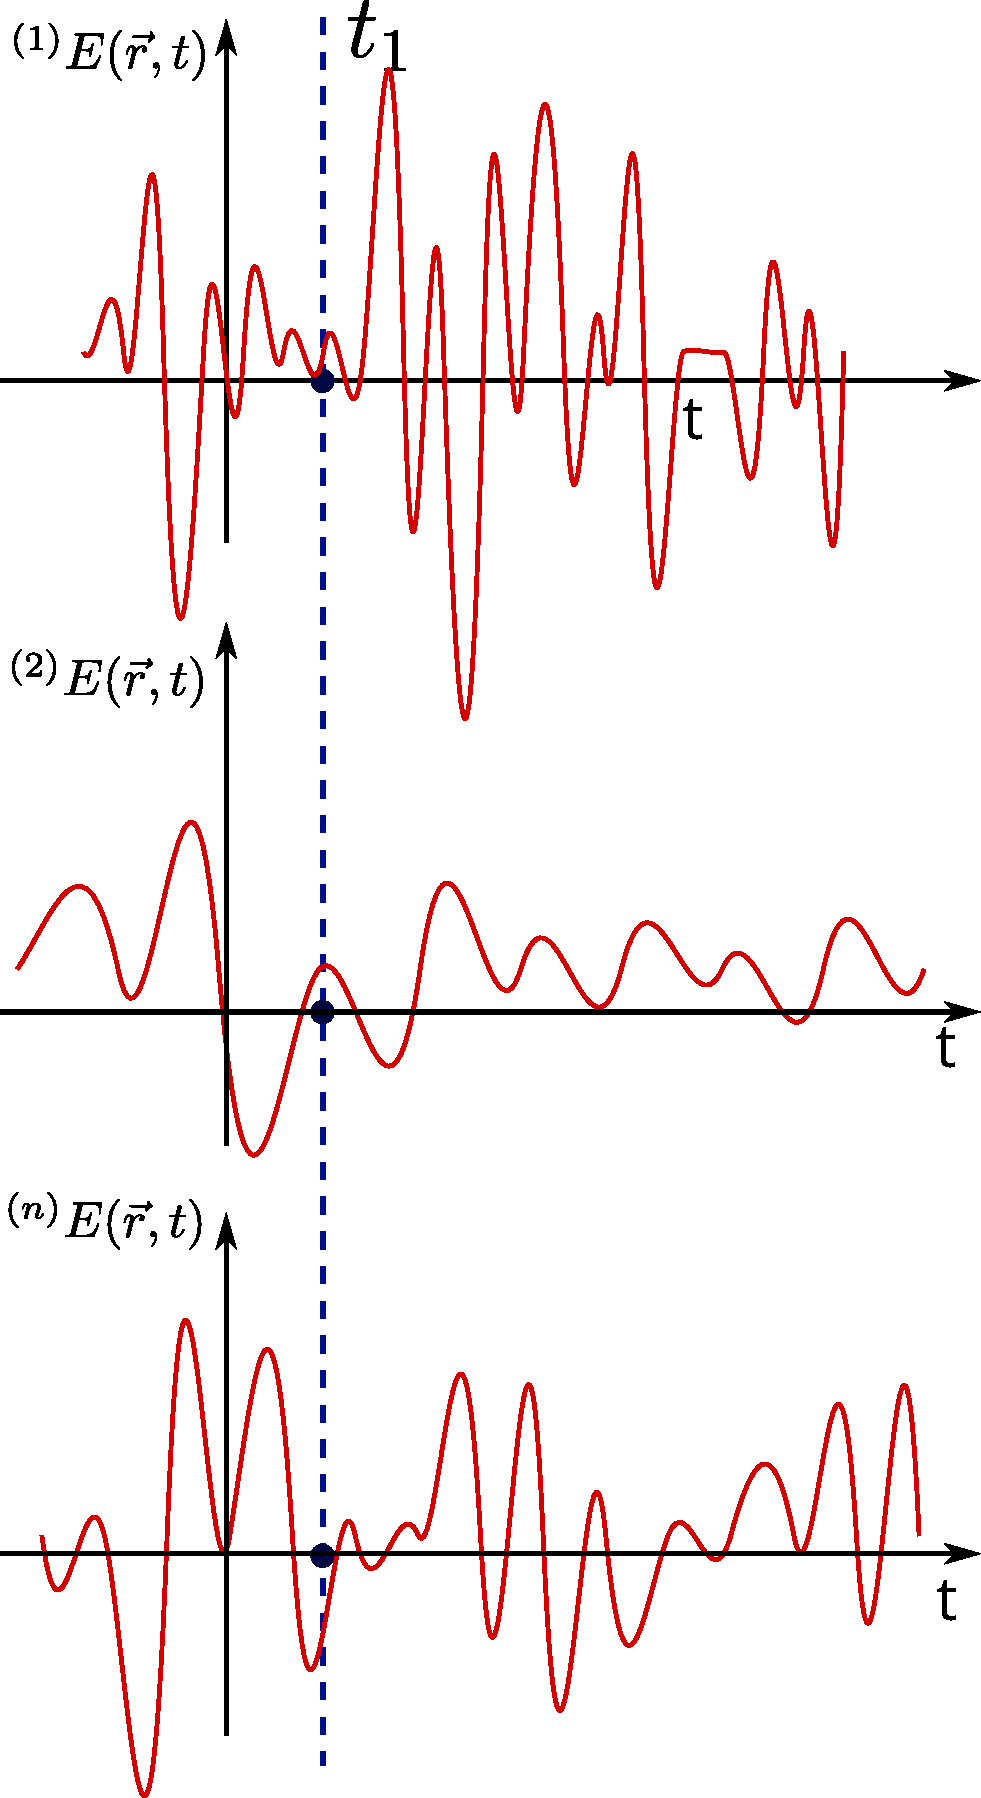
\includegraphics[width=0.4\linewidth]{Capitulo 2/Figuras/RandomVar}
		\caption{Representación de $E(\vec{r},t)$ como una variable aleatoria.}
		\label{fig:randomvar}
	\end{figure}

	En la Figura~\ref{fig:randomvar} observamos una componente del campo eléctrico, representada por $E(\vec{r},t)$, vista a través de varias observaciones o realizaciones. Comportándose como una variable aleatoria, en cada realización tiene un comportamiento distinto en el tiempo en un punto $\vec{r}$; en general, aquí hemos indexado $^{(i)}E(\vec{r},t)$ con enteros, pero en general podría haber un conjunto no numerable de estados posibles para el campo eléctrico. Si observamos la Figura~\ref{fig:randomvar} hay dos puntos temporales, $t,t'$, en los que aislamos partes de estas oscilaciones aleatorias; podríamos preguntar cuán correlacionadas están estas oscilaciones a través de las realizaciones a lo largo del intervalo $t'-t$, o dicho de otro modo, cuán \textit{coherentes} son las oscilaciones a través de las realizaciones.

	Hablamos de coherencia cuando queremos analizar la correlación de la radiación electromagnética entre puntos del espaciotiempo. Si tenemos dos fuentes que emiten un campo eléctrico (por el momento entendido como escalar), su función de coherencia viene dada por

	\begin{equation}
		\Gamma(\vec{r},\vec{r}';t,t') = E \left\{ \mathcal{E} (\vec{r},t) \mathcal{E}^*(\vec{r}',t') \right\},
	\end{equation}

	donde estamos calculando el promedio de ensamble de las componentes $\mathcal{E}$, que son números complejos como ya se discutió en estos apuntes. Si tomamos $\vec{r}=\vec{r}'$ obtenemos lo que se conoce como la \textit{función de coherencia mutua}

	\begin{equation}
		\Gamma(\vec{r}';t,t') = E \left\{ \mathcal{E}(\vec{r}',t) \mathcal{E}^*(\vec{r}',t') \right\}.
	\end{equation}

	Podemos ir aún más lejos incluyendo el concepto de \textit{estacionariedad estadística}, pero hay que tener cuidado pues existen varios tipos. Formalmente, un proceso estocástico $\{X_t\}$ se considera estacionario cuando sus propiedades estadísticas son invariantes bajo traslaciones temporales. Esta condición se manifiesta en distintos grados:

	\begin{enumerate}
		\item \textbf{Estacionariedad estricta (fuerte)}: la forma más exigente de estacionariedad requiere que todas las distribuciones de probabilidad conjuntas sean invariantes en el tiempo:

		\begin{equation}
			F_X(x_{t_1+\tau}, \ldots, x_{t_k+\tau}) = F_X(x_{t_1}, \ldots, x_{t_k}) \quad \forall \tau, k, t_i,
		\end{equation}
		donde $F_X$ es la función de distribución conjunta. Esto implica que:
		\begin{itemize}
			\item todos los momentos (media, varianza, asimetría, etc.) son constantes;
			\item las distribuciones marginales son idénticas en cualquier instante;
			\item es una condición suficiente pero no necesaria para los modelos ARMA.
		\end{itemize}

		\item \textbf{Estacionariedad débil (de segundo orden)}: más práctica en las aplicaciones, solo requiere la invariancia de los dos primeros momentos:
		\begin{equation}
			\begin{cases}
				\mathbb{E}[X_t] = \mu \quad (\text{constante}) \quad \forall t \\
				\text{Var}(X_t) = \sigma^2 \quad (\text{constante}) \quad \forall t \\
				\text{Cov}(X_t, X_{t+h}) = \gamma(h) \quad (\text{depende solo de } h, \text{ no de } t)
			\end{cases}
		\end{equation}
		Esta es la definición usada en la mayoría de los modelos econométricos (ARIMA, GARCH) y en el análisis espectral de Wiener-Khinchin (que usaremos más adelante).

		\item \textbf{Estacionariedad de tendencia (estacionariedad determinista)}: un proceso no estacionario que puede volverse estacionario removiendo componentes deterministas:
		\begin{equation}
			X_t = \alpha + \beta t + \epsilon_t,
		\end{equation}
		donde $\epsilon_t$ es estacionario. La no estacionariedad aquí proviene exclusivamente de la tendencia temporal $\beta t$.
	\end{enumerate}

	Usaremos una hipótesis de estacionariedad fuerte (aunque a menudo basta con la estacionariedad débil). En este espíritu, si $\tau = t-t'$ tenemos

	\begin{equation}
		\Gamma(\vec{r}',t,t') = \Gamma(\vec{r}',t-t') = \Gamma(\vec{r}',\tau).
	\end{equation}

	Como podemos ver, la coherencia mutua en un punto $\vec{r}'$ bajo una hipótesis de estacionariedad da lugar a una dependencia explícita en la diferencia temporal $\tau$ dentro del promedio de ensamble.

	Vale la pena preguntarse: ¿cuán necesario es analizar el promedio de ensamble; por qué no tomar el promedio temporal? Responder esto es \textit{muy complicado}, pues toca el problema de la \textit{ergodicidad}. La ergodicidad, en el sentido de la teoría ergódica, requiere que un sistema dinámico satisfaga que los promedios temporales coincidan con los promedios espaciales para casi toda condición inicial. Su demostración rigurosa es altamente no trivial, hasta el punto de que los problemas para los cuales la ergodicidad se ha demostrado con rigor matemático son pocos.

	Desde un punto de vista fenomenológico asumiremos, de aquí en adelante, una \textit{hipótesis ergódica} en la cual la radiación electromagnética tiene un carácter estacionario y ergódico. Bajo estas condiciones la función de coherencia mutua coincide con el promedio temporal

	\begin{equation}
		\Gamma(\vec{r}';t,t') = \int_{\mathbb{R}} \mathcal{E}(\vec{r}',t') \mathcal{E}^*(\vec{r}',t-t')\,dt'.
	\end{equation}

	La función de coherencia mutua tiene varias propiedades, algunas de las cuales son:

	\begin{itemize}
		\item[a)] $\Gamma(\vec{r}',0) \geq 0$. Esto se sigue de la definición, pues $\Gamma(\vec{r}',0) = \braket{|\mathcal{E}(\vec{r}')|^2}$, es decir, corresponde a la intensidad del campo eléctrico y solo puede anularse cuando trivialmente el campo es nulo en todo instante.

		\item[b)] $\Gamma(\vec{r}',-\tau) = \Gamma^*(\vec{r}',\tau)$. Esto se conoce como la \textit{propiedad hermítica} de la función de coherencia mutua, y se sigue del hecho de que $\mathcal{E}(\vec{r}',t)$ es estacionario, lo cual permite traslaciones temporales arbitrarias desde el origen. En este espíritu,

		\begin{align}
			& \Gamma(\vec{r}',\tau) = \braket{\mathcal{E}(\vec{r}')\mathcal{E}^*(\vec{r}',t + \tau)} = \braket{\mathcal{E}(\vec{r}',t-\tau)\mathcal{E}^*(\vec{r}')} = \Gamma^*(\vec{r}',-\tau).
		\end{align}

		\item[c)] $|\Gamma(\vec{r}',\tau)| \leq \Gamma(\vec{r}',0)$. Esta propiedad se sigue de la \textit{desigualdad de Cauchy-Schwarz}

		\begin{equation}
			|\Gamma(\vec{r}',\tau)|^2 = | \braket{\mathcal{E}(\vec{r}')\mathcal{E}^*(\vec{r}',t+\tau)} |^2 \leq  \braket{\mathcal{E}(\vec{r}',t)\mathcal{E}^*(\vec{r}',t)} \braket{\mathcal{E}(\vec{r}',t+\tau)\mathcal{E}^*(\vec{r}',t+\tau)} = \Gamma^2(\vec{r}',0),
		\end{equation}

		lo cual implica que $|\Gamma(\vec{r}',\tau)|$ jamás puede exceder su valor inicial $\Gamma(\vec{r}',0)$. (Esta propiedad es, recordemos, exclusiva de la función de coherencia mutua; cuando consideremos la coherencia entre dos fuentes veremos que no se cumple, sino que, por el contrario, aumentará.)

		\item[d)] $\Gamma(\vec{r}',\tau)$ es no negativa. Podemos ver esto a partir de la definición mediante la siguiente desigualdad, bastante obvia,

		\begin{equation}
			\left\langle \left| \int_{T_1}^{T_2} f(t)\mathcal{E}(t)\,dt \right|^2\right\rangle \geq 0,
		\end{equation}
		donde $f(t)$ es una función arbitraria y $T_1,T_2$ son instantes arbitrarios. De este modo obtenemos la desigualdad

		\begin{equation}
			\int_{T_1}^{T_2}\int_{T_1}^{T_2} f^*(\vec{r}',t)f(\vec{r}',t')\Gamma(\vec{r}',t'-t)\,dt\,dt' \geq 0.
		\end{equation}

		\item[e)] Si el campo eléctrico es aleatorio, estacionario y diferenciable, entonces podemos hallar una velocidad $\xi (\vec{r}',t) = \dot{\mathcal{E}}(\vec{r}',t)$, que es estacionaria, aleatoria y de valor medio nulo, y cuya función de coherencia mutua es

		\begin{equation}
			\Gamma_\xi(\vec{r}',\tau) = - \ddot{\Gamma}_\mathcal{E}(\vec{r}',\tau).
		\end{equation}

		\item[f)] $\Gamma(\vec{r}',\tau)$ es continua. Esto se cumple incluso cuando hay discontinuidades de salto.
	\end{itemize}

	Finalmente, vale la pena mencionar que existe una cantidad conocida como el grado complejo de coherencia, dada por

	\begin{equation}
		\gamma (\vec{r}',\tau) = \frac{\Gamma(\vec{r}',\tau)}{\Gamma(\vec{r}',0)},
	\end{equation}

	y a partir de la desigualdad de Cauchy-Schwarz tenemos $0 \leq |\gamma(\vec{r}',\tau)| \leq 1$.

	\subsection{Manifestaciones de la coherencia: el teorema de Wiener-Khinchin}

		La función de coherencia mutua y la densidad espectral de potencia son dos caras de la misma moneda en el estudio de la luz y las señales ondulatorias. La coherencia mutua describe cómo se correlacionan las fluctuaciones de un campo luminoso en el espacio y en el tiempo, actuando como un mapa que revela hasta qué punto las variaciones en un punto del espacio están sincronizadas con las de otro, incluso con cierto retardo temporal. La densidad espectral de potencia, a su vez, descompone la energía de la señal en sus componentes de frecuencia, mostrando qué tonos o colores —en el caso de la luz— dominan su comportamiento. La relación íntima entre ambos conceptos radica en que, mediante transformaciones matemáticas, es posible convertir la información detallada sobre las correlaciones espaciotemporales capturada por la coherencia mutua en una descripción precisa de cómo se distribuye la energía en el dominio de la frecuencia, y viceversa. Este vínculo permite saltar entre perspectivas complementarias: analizar patrones de interferencia en un interferómetro o identificar firmas espectrales en un material, todo a partir de los mismos principios fundamentales.

		Vamos a encontrar uno de los teoremas más importantes de la teoría de la coherencia, el \textit{teorema de Wiener-Khinchin}. Nótese que las señales aleatorias estacionarias no tienen transformada de Fourier; por ello podemos definir las siguientes señales aleatorias truncadas del campo eléctrico

		\begin{equation}\label{eq:NearlyWiener}
			^\omega \mathcal{E}_T (\vec{r},t) = \left\{
			\begin{matrix}
				^\omega\mathcal{E}(\vec{r},t) & -\frac{T}{2}\leq t \leq \frac{T}{2}\\
				0 & \text{en otro caso}
			\end{matrix} \right.
		\end{equation}

		y definimos la potencia espectral para una realización $\omega$ como la magnitud al cuadrado de las transformadas de Fourier de los campos eléctricos \eqref{eq:NearlyWiener}, es decir,

		\begin{equation}\label{eq:SpecWT}
			^\omega S_T (\vec{r},\nu) = \left| \int_\mathbb{R} ^\omega \mathcal{E}_T(\vec{r},t)e^{i2\pi\nu t}dt \right|^2 = \left| \int_{-T/2}^{T/2}\;^\omega \mathcal{E}(\vec{r},t)e^{i2\pi\nu t}dt \right|^2,
		\end{equation}

		y la \textit{densidad espectral de potencia del evento} $\omega$ la calculamos como

		\begin{equation}\label{eq:SpecW}
			\lim_{T \to \infty} \frac{^\omega S_T(\vec{r},\nu)}{T} = {}^\omega S(\vec{r},\nu).
		\end{equation}

		Puesto que ya poseemos una herramienta para estudiar, en cada evento o realización, la densidad espectral de potencia, entonces, mediante su promedio de ensamble, podemos hallar la densidad total, es decir,

		\begin{equation}
			S(\vec{r},\nu) = E\left\{^\omega S(\vec{r},\nu)\right\},
		\end{equation}

		introduciendo las ecuaciones \eqref{eq:SpecWT} y \eqref{eq:SpecW} tenemos entonces

		\begin{align}
			& S(\vec{r},\nu) = E\left\{ \lim_{T \to \infty} \left| \frac{1}{T} \int_{-T/2}^{T/2}\;^\omega \mathcal{E}(\vec{r},t)e^{i2\pi\nu t}dt \right|^2 \right\},\\
			& S(\vec{r},\nu) = \lim_{T \to \infty} \frac{1}{T}  \int_{-T/2}^{T/2}\int_{-T/2}^{T/2} E \left\{ \mathcal{E}(\vec{r},t)\mathcal{E}^*(\vec{r}',t') \right\} e^{i2\pi\nu(t-t')}dt\,dt',\\
			& S(\vec{r},\nu) = \int_{\mathbb{R}}\Gamma(\vec{r},\vec{r}';\tau)e^{i2\pi\nu \tau}d\tau,
		\end{align}

		\begin{equation}\label{eq:WienerKhinchin}
			\boxed{S(\vec{r},\nu) = \mathcal{F}\left\{ \Gamma(\vec{r},\vec{r}',\tau) \right\}}.
		\end{equation}

		El resultado \eqref{eq:WienerKhinchin} se lee: la transformada de Fourier de la función de coherencia corresponde a la densidad espectral de potencia, y se conoce como el teorema de Wiener-Khinchin. Su uso es fundamental, pues nos dice que mediante métodos como la espectrometría podemos hallar la función de coherencia de cualquier fenómeno; podemos incluso ir más lejos, ya que este resultado en realidad se desprende de algo más general —la función de correlación—, lo que significa que todo fenómeno estocástico tiene un espectro asociado, y a partir de las mediciones o estimaciones de ese espectro podemos calcular las correlaciones del sistema.

		Si hacemos una observación simple, el rango óptico de la radiación —el visible— es una banda de frecuencias muy bajas respecto de todo el espectro; el visible va aproximadamente de $400$~nm a $700$~nm, y podemos decir que toda la óptica es de \textit{banda angosta}. Esto obedece la desigualdad

		\begin{equation}
			\frac{\triangle \nu}{\nu} \ll 1,
		\end{equation}

		y, en este régimen de banda angosta, la función de coherencia toma la forma

		\begin{equation}
			\Gamma(\vec{r};\tau) = \tilde{\Gamma}(\vec{r})e^{i2\pi \tilde{\nu}\tau},
		\end{equation}

		lo cual podemos representar gráficamente como se muestra en la Figura~\ref{fig:narrow}, donde se puede ver el comportamiento de la función de coherencia en el régimen de banda angosta.\footnote{Suele encontrarse en la literatura un término parecido pero no igual al de banda angosta, conocido como la condición de cuasimonocromaticidad, escrita como $\frac{\triangle \lambda}{\lambda} \ll 1$; pero esto acota la longitud de onda para que sea lo más monocromática posible, mientras que la condición de banda angosta admite varias frecuencias, siempre que sean angostas respecto de todo el espectro de frecuencias.} Allí se observa una envolvente (lo observable) que envuelve todas las frecuencias fundamentales.

		\begin{figure}[htbp]
			\centering
			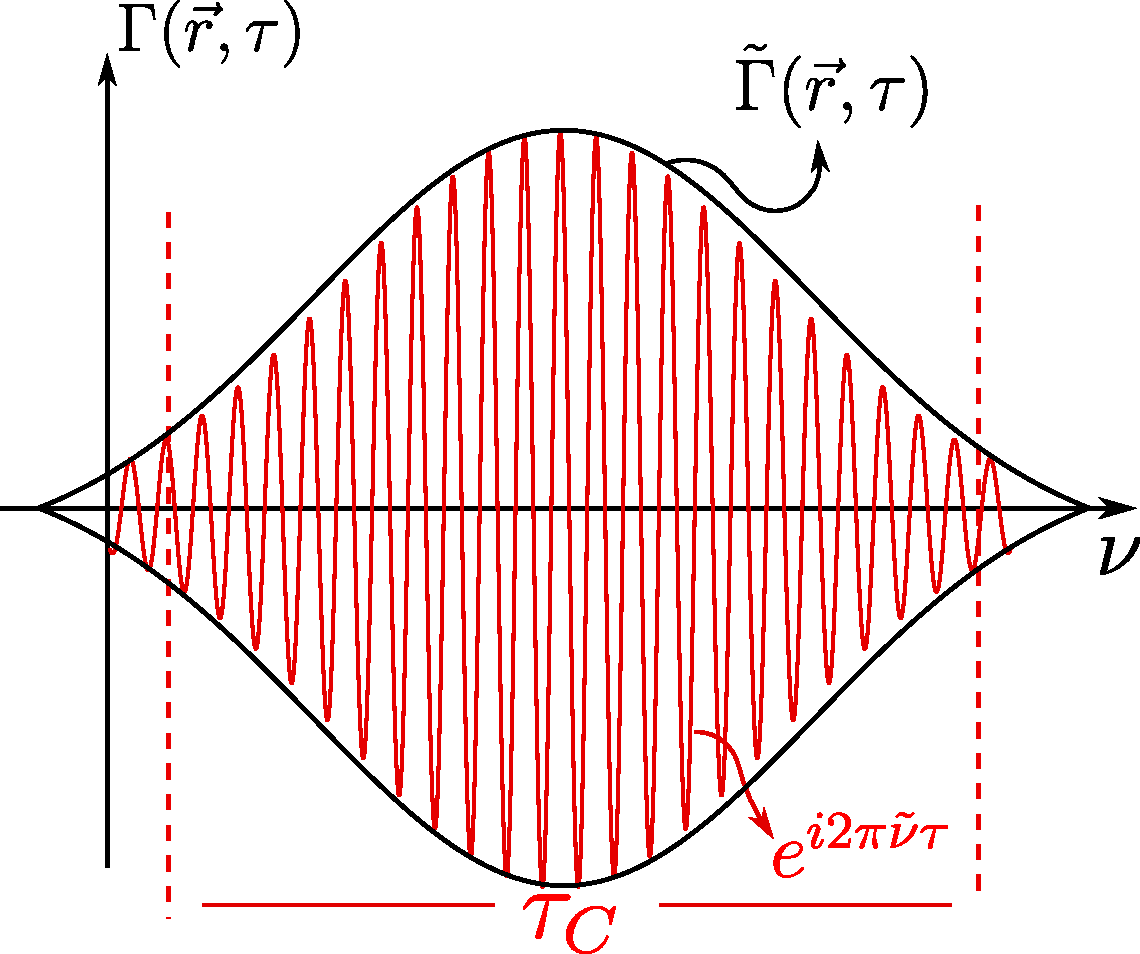
\includegraphics[width=0.7\linewidth]{Capitulo 2/Figuras/Estrecho}
			\caption{Representación gráfica de la función de coherencia de banda angosta. En negro se muestra la envolvente $\tilde{\Gamma}(\vec{r},\tau)$, y en rojo las oscilaciones $e^{i2\pi\tilde{\nu}\tau}$. Estas oscilaciones están confinadas dentro de algo conocido como el tiempo de coherencia $\tau_C$, que veremos más adelante.}
			\label{fig:narrow}
		\end{figure}

	\subsection{Ecuación de onda de la coherencia}

		Salgamos un poco de la zona de confort y comprendamos cómo se propagan las correlaciones a través del espacio y del tiempo. Sea $\mathcal{E}^{(r)}(\vec{r},t)$ alguna componente \textit{real} del campo eléctrico, vista como una señal aleatoria. Como es bien sabido a partir de la teoría electromagnética clásica, obedece las ecuaciones de Maxwell y por tanto tiene asociada una ecuación de onda, a saber

		\begin{equation}
			\nabla^2 \mathcal{E}^{(r)}(\vec{r},t) = \frac{1}{C^2}\frac{\partial^2 \mathcal{E}^{(r)}(\vec{r},t)}{\partial t^2},
		\end{equation}

		donde $C$ es la velocidad de la luz en el vacío. También tenemos, por análisis de Fourier,

		\begin{equation}\label{eq:EandFourier}
			\mathcal{E}(\vec{r},t) = \int_0^{\infty} \tilde{\mathcal{E}}(\vec{r},\nu) e^{-i2\pi\nu t}d\nu .
		\end{equation}

		Y si aplicamos el operador d'alembertiano $\square = \nabla^2 - \frac{1}{C^2}\frac{\partial^2}{\partial t^2}$ a la ecuación \eqref{eq:EandFourier}, encontramos que $\tilde{\mathcal{E}}(\vec{r},\nu)$ tiene la forma de una ecuación de tipo Helmholtz, es decir,

		\begin{equation}
			\nabla^2 \mathcal{E}(\vec{r},t) - \frac{1}{C^2}\frac{\partial^2 \mathcal{E}(\vec{r},t)}{\partial t^2} = \int_0^{\infty} \left[ \nabla^2 \tilde{\mathcal{E}}(\vec{r},\nu) + k^2 \tilde{\mathcal{E}}(\vec{r},\nu) \right]e^{-i2\pi\nu t}d\nu,
		\end{equation}

		lo que nos lleva al hecho de que el campo eléctrico, como señal analítica y compleja, también obedece una ecuación de tipo ondulatorio

		\begin{equation}
			\nabla^2 \mathcal{E}(\vec{r},t) = \frac{1}{C^2}\frac{\partial^2 \mathcal{E}(\vec{r},t)}{\partial t^2}.
		\end{equation}

		Tomando el complejo conjugado de la ecuación anterior tenemos

		\begin{equation}\label{eq:NearlyWaveForE}
			\nabla^2 \mathcal{E}^*(\vec{r},t) = \frac{1}{C^2}\frac{\partial^2 \mathcal{E}^*(\vec{r},t)}{\partial t^2}.
		\end{equation}

		Si multiplicamos ambos lados de la ecuación \eqref{eq:NearlyWaveForE} por $\mathcal{E}(\vec{r}',t')$, y dado que hemos tomado el d'alembertiano respecto de las variables sin prima, usando algunas reglas de signos tenemos

		\begin{equation}\label{eq:NoAvg}
			\nabla^2 \left[ \mathcal{E}^*(\vec{r},t)\mathcal{E}(\vec{r}',t') \right] =  \frac{1}{C^2} \frac{\partial^2}{\partial t^2}\left[ \mathcal{E}^*(\vec{r},t)\mathcal{E}(\vec{r}',t') \right].
		\end{equation}

		Tomando el promedio de ensamble de la ecuación \eqref{eq:NoAvg} sobre todas las realizaciones del campo, esta ecuación de onda se convierte en

		\begin{equation}\label{eq:coherenceWave1}
			\nabla^2 \Gamma(\vec{r},\vec{r}';t,t') = \frac{1}{C^2}\frac{\partial^2}{\partial t^2} \Gamma(\vec{r},\vec{r}';t,t'),
		\end{equation}

		y, de manera análoga, usando $\square' = \nabla'^2 - \frac{1}{C^2}\frac{\partial^2}{\partial t'^2}$ tenemos otra ecuación de onda dada por

		\begin{equation}\label{eq:coherenceWave2}
			\nabla'^2 \Gamma(\vec{r},\vec{r}';t,t') = \frac{1}{C^2}\frac{\partial^2}{\partial t'^2} \Gamma(\vec{r},\vec{r}';t,t').
		\end{equation}

		Las ecuaciones \eqref{eq:coherenceWave1} y \eqref{eq:coherenceWave2} nos dicen directamente que las funciones de coherencia entre dos puntos del espaciotiempo evolucionan en el tiempo siguiendo una ecuación de tipo ondulatorio, por separado, respecto de cada par de coordenadas espaciotemporales —un resultado que es, sin duda, notable—. Podemos llevar este resultado aún más lejos y estudiar esta propagación en la siguiente sección.

	\subsection{Propagación de la coherencia y la dirección del tiempo: el teorema de van Cittert-Zernike}

		\begin{figure}[htbp]
			\centering
			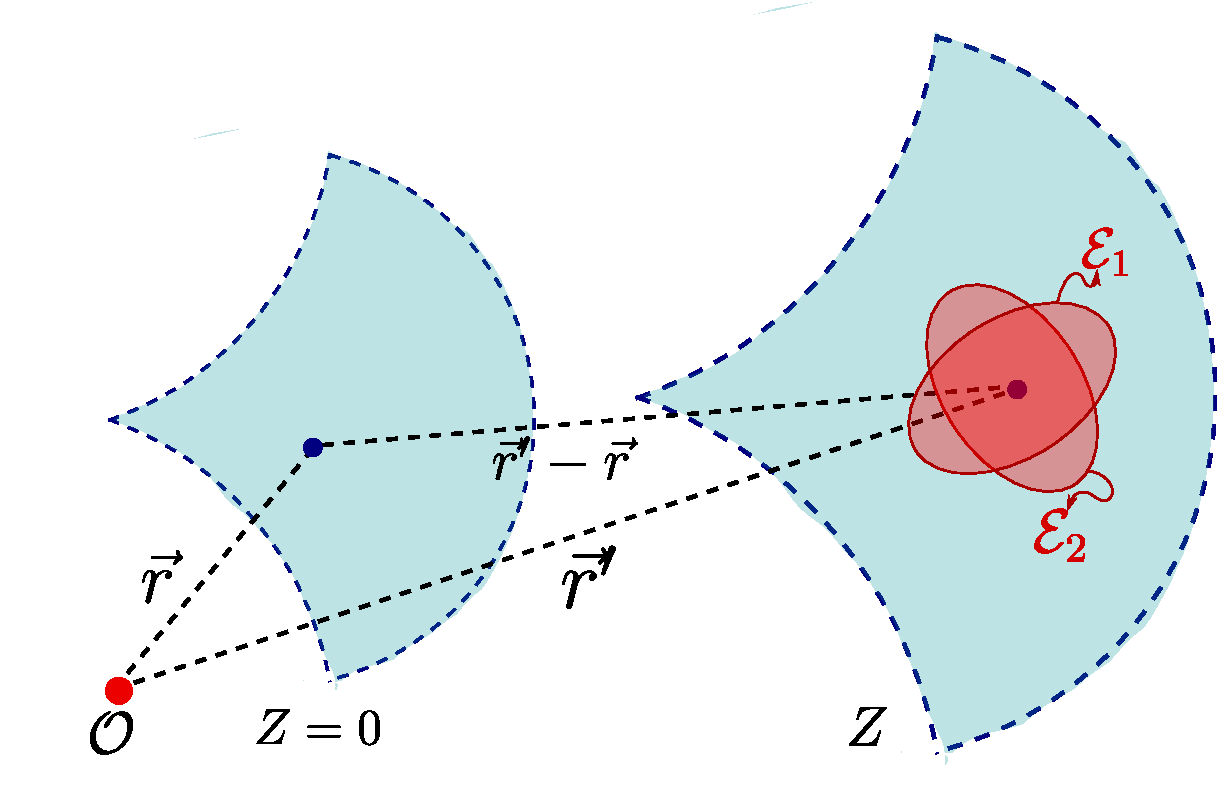
\includegraphics[width=0.8\linewidth]{Capitulo 2/Figuras/Propagation}
			\caption{Propagación del campo eléctrico desde un plano $Z=0$ hasta un plano $Z$, donde cada punto del frente de onda lleva su elipse de polarización media.}
			\label{fig:propagation}
		\end{figure}

		Como sabemos, el campo eléctrico obedece una ecuación de tipo ondulatorio y la orientación de los campos viene dada por la polarización del campo; a su vez, como vimos en el capítulo de difracción (véase la Sección~\ref{Sec:Diffraction}), a nivel clásico la luz se propaga fundamentalmente como ondas esféricas, tal como se ilustra en la Figura~\ref{fig:propagation}, y en cada punto del frente de onda las componentes del campo eléctrico oscilan aleatoriamente, pero dentro de la elipse de polarización media de su estado representativo. Matemáticamente podemos representar esta componente como

		\begin{equation}
			\mathcal{E}_z(\vec{r}_1,\nu) = \frac{i}{\lambda} \int_{\Sigma} \mathcal{E}_0 (\vec{r},\nu) \frac{e^{ik \|\vec{r}_1-\vec{r}\|}}{\|\vec{r}_1-\vec{r}\|}\cos(\hat{z}; \vec{r}_1-\vec{r})\,d\sigma .
		\end{equation}

		Usando la ecuación \eqref{eq:EandFourier} tenemos

		\begin{equation}
			\mathcal{E}_z(\vec{r}_1,t) = \frac{1}{i}\int_{\mathbb{R}^+} \frac{\nu}{V} \int_{\Sigma} \mathcal{E}_0(\vec{r},\nu)\frac{\cos\left(  \hat{z}; \vec{r}_1 - \vec{r} \right)}{\|\vec{r}_1 - \vec{r}\|} e^{i2\pi \nu \left( t + \frac{\|\vec{r}_1 - \vec{r}\|}{V} \right)} d\sigma\, d\nu,
		\end{equation}

		donde $V$ es la velocidad de propagación de la envolvente. Reescribiendo un poco más, tenemos

		\begin{equation}
			\mathcal{E}_z(\vec{r}_1,t) = \frac{1}{i} \int_{\Sigma} \frac{\cos\left( \hat{z}; \vec{r}_1-\vec{r} \right)}{\|\vec{r}_1 -\vec{r}\|} \int _{\mathbb{R}^+} \frac{\nu}{V} \mathcal{E}_0 (\vec{r},\nu)e^{i2\pi\nu \left(t + \frac{\|\vec{r}_1 - \vec{r}\|}{V}\right)}d\nu\, d\sigma,
		\end{equation}

		y, tomando la aproximación de banda angosta, tenemos

		\begin{equation}\label{eq:IntegralEz}
			\mathcal{E}_z(\vec{r}_1,t) = \frac{1}{i\tilde{\lambda}} \int_{\Sigma} \mathcal{E}_0 \left(\vec{r}, t +\frac{\|\vec{r}_1 - \vec{r}\|}{V}\right) \frac{\cos\left(\hat{z} ; \vec{r}_1 - \vec{r}\right)}{\|\vec{r}_1-\vec{r}\|} d\sigma .
		\end{equation}

		Podemos visualizar gráficamente cómo pretendemos propagar en la Figura~\ref{fig:propagation2}, donde observamos que estamos partiendo de la función de coherencia entre dos puntos $\vec{r},\vec{r}'$ en los instantes $t,t'$, respectivamente, y llevándola hasta una función de coherencia en los puntos $\vec{r}_1,\vec{r}_2$ en dos instantes $t_1,t_2$, respectivamente.

		\begin{figure}[htbp]
			\centering
			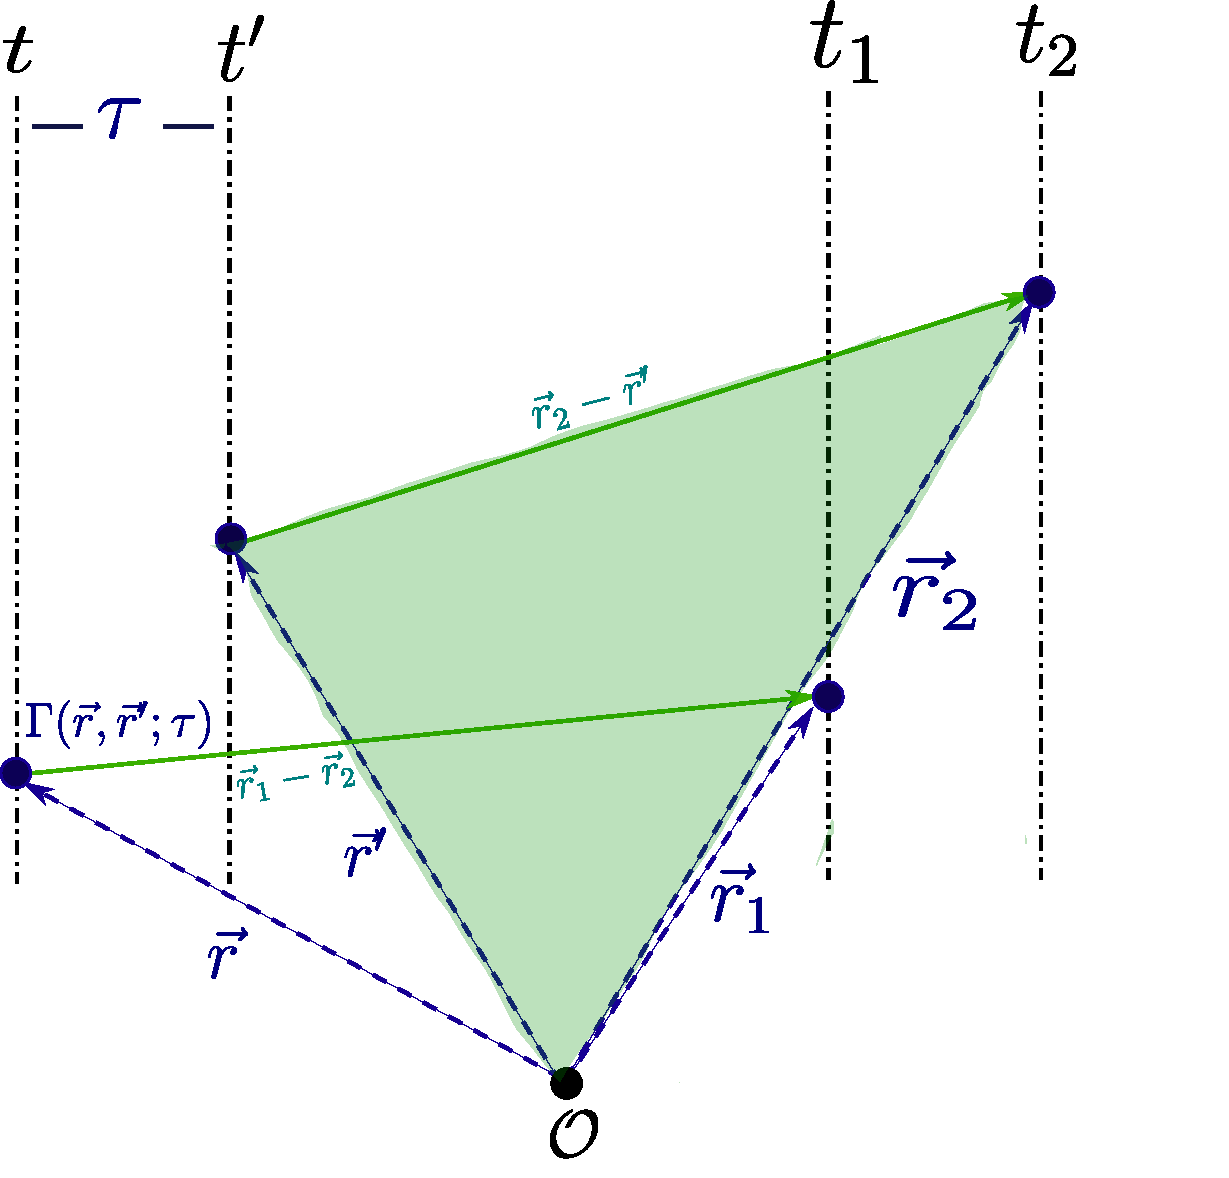
\includegraphics[width=0.8\linewidth]{Capitulo 2/Figuras/Propagation2}
			\caption{Propagación de la función de coherencia entre dos puntos $\vec{r},\vec{r}'$ en el plano inicial hasta la coherencia entre dos puntos $\vec{r}_1,\vec{r}_2$ en el plano de observación.}
			\label{fig:propagation2}
		\end{figure}

		Partiendo de la ecuación \eqref{eq:IntegralEz} podemos calcular la función de coherencia en su propagación como

		\begin{equation}
			\Gamma_z(\vec{r}_1,\vec{r}_2;\tau) = E \left\{ \mathcal{E}_z(\vec{r}_1,t) \mathcal{E}_z^*(\vec{r}_2,t-\tau) \right\},
		\end{equation}

		\begin{align}
			&\Gamma_z(\vec{r}_1,\vec{r}_2;\tau) = E\left\{\frac{1}{i\tilde{\lambda}} \int_{\Sigma} \mathcal{E}_0 \left(\vec{r},t + \frac{\|\vec{r}_1 - \vec{r}\|}{V}\right) \frac{\cos\left(\hat{z};\vec{r}_1-\vec{r}\right)}{\|\vec{r}_1-\vec{r}\|}d\sigma \right. \\
			& \left. \cdot \frac{1}{-i\tilde{\lambda}} \int_{\Sigma'} \mathcal{E}_0^* \left(\vec{r}',t - \tau + \frac{\|\vec{r}_2 - \vec{r}'\|}{V}\right) \frac{\cos\left(\hat{z};\vec{r}_2-\vec{r}'\right)}{\|\vec{r}_2-\vec{r}'\|}d\sigma'  \right\},
		\end{align}

		\begin{align}
			& \Gamma_z(\vec{r}_1,\vec{r}_2;\tau) = \frac{1}{\tilde{\lambda}^2} \int_{\Sigma}\int_{\Sigma'} E \left\{ \mathcal{E}_0\left(\vec{r}, t + \frac{\|\vec{r}_1 - \vec{r}\|}{V}\right) \mathcal{E}_0^* \left(\vec{r}', t-\tau + \frac{\|\vec{r}_2 - \vec{r}'\|}{V}\right) \right\}\frac{\cos \left(\hat{z};\vec{r}_1-\vec{r}\right) \cos\left(\hat{z}; \vec{r}_2 - \vec{r}' \right) }{\|\vec{r}_2-\vec{r}'\|\cdot \|\vec{r}_1 - \vec{r}\|} d\sigma\, d\sigma',
		\end{align}

		\begin{equation}\label{eq:IntGamma}
			\Gamma_z (\vec{r}_1,\vec{r}_2;\tau) = \frac{1}{\tilde{\lambda}^2}\int_{\Sigma}\int_{\Sigma'} \Gamma_0 \left(\vec{r},\vec{r}';\tau + \frac{\|\vec{r}_1 - \vec{r}\| + \|\vec{r}_2 - \vec{r}'\|}{V}\right) \frac{\cos \left(\hat{z};\vec{r}_1-\vec{r}\right) \cos\left(\hat{z}; \vec{r}_2 - \vec{r}' \right) }{\|\vec{r}_2-\vec{r}'\|\cdot \|\vec{r}_1 - \vec{r}\|} d\sigma\, d\sigma'
		\end{equation}

		\begin{figure}[htbp]
			\centering
			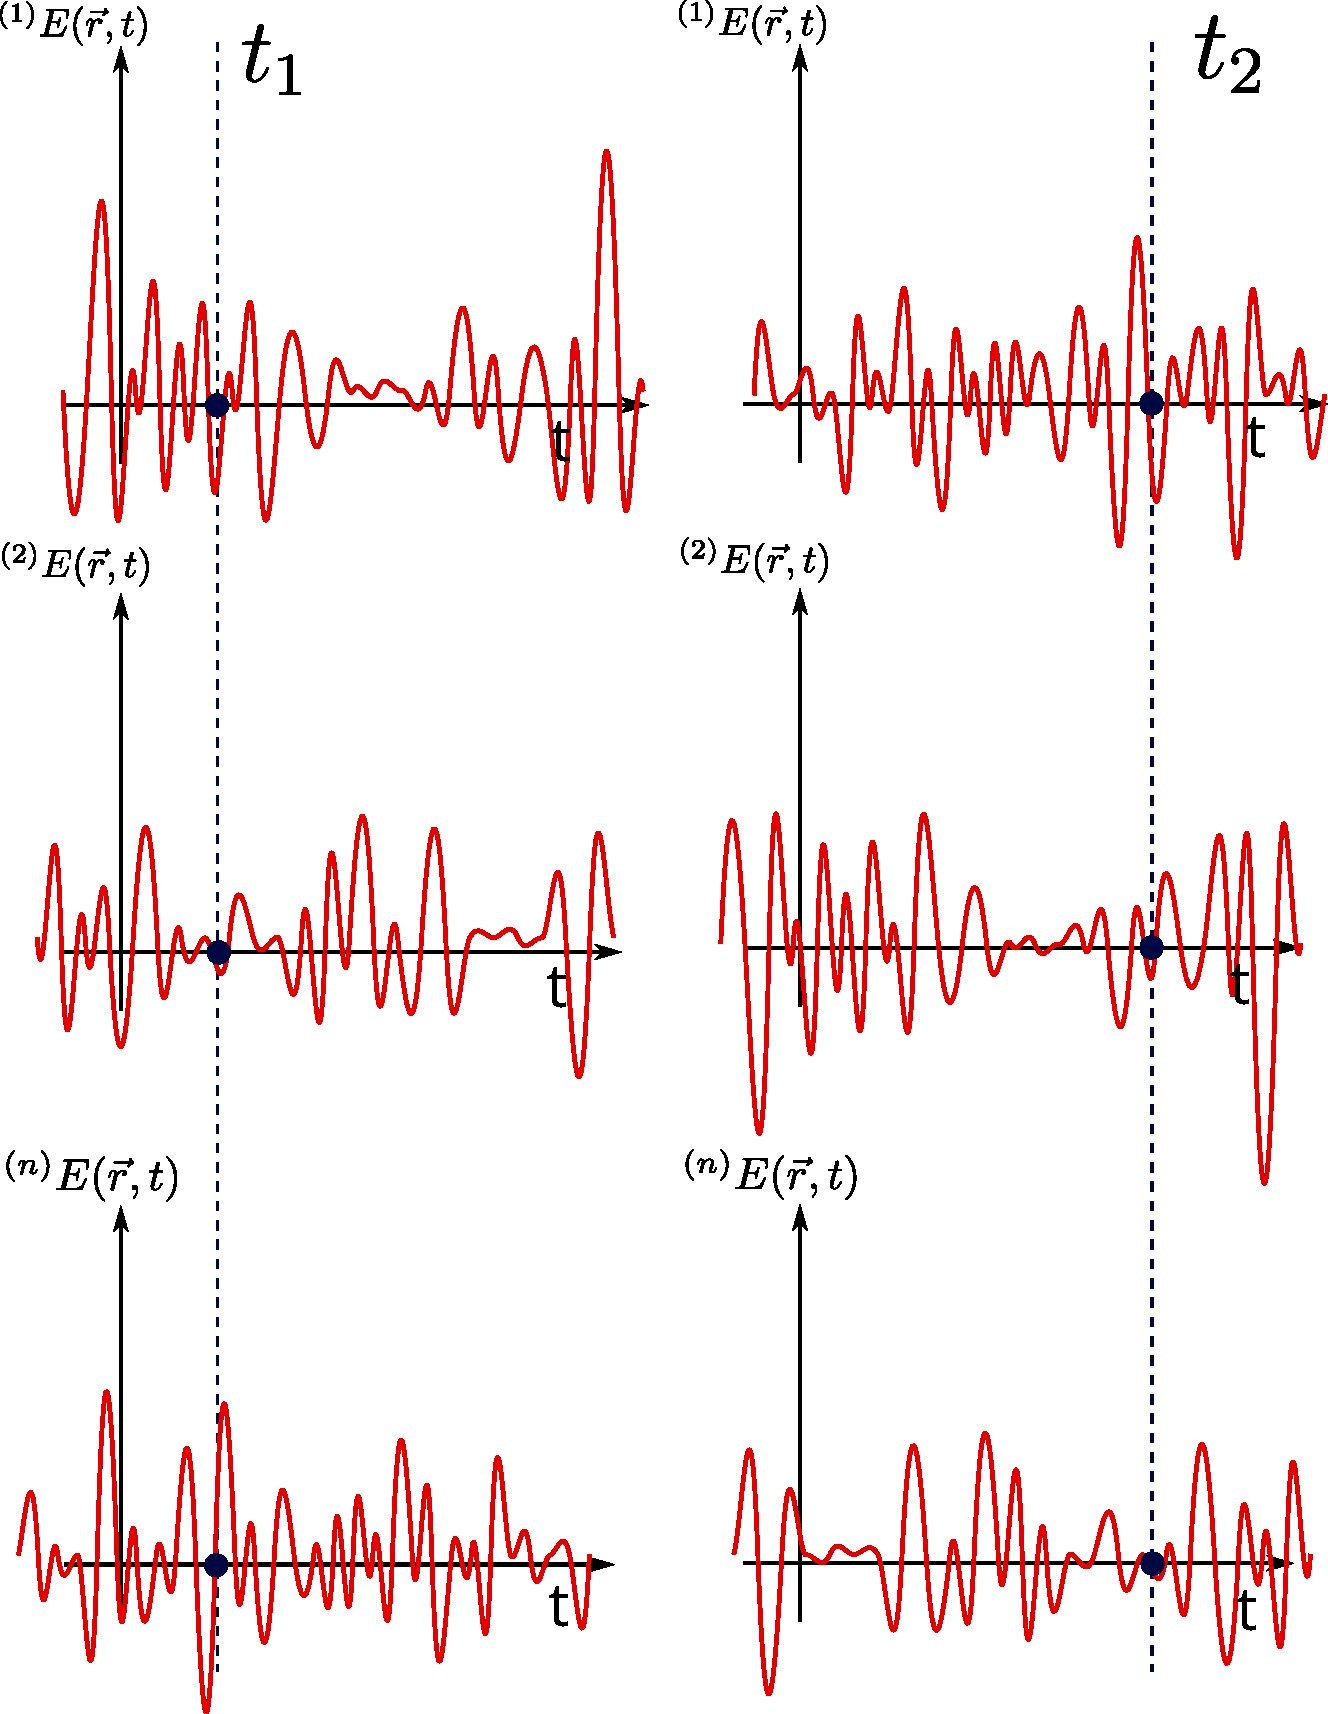
\includegraphics[width=0.6\linewidth]{Capitulo 2/Figuras/Random2}
			\caption{Evolución de las realizaciones al propagar el campo eléctrico.}
			\label{fig:random2}
		\end{figure}

		La propagación de las oscilaciones aleatorias a través de $n$ realizaciones puede visualizarse en la Figura~\ref{fig:random2}.

		Vamos a imponer la siguiente condición sobre la función de coherencia

		\begin{equation}
			\Gamma(\vec{r},\vec{r}';\tau) = \Gamma(\vec{r}';\tau) \delta(\vec{r}-\vec{r}'),
		\end{equation}

		lo cual, en pocas palabras, significa que, espacialmente hablando, la distribución que representa la función de coherencia está localizada en un punto y ponderada por la coherencia mutua en el punto $\vec{r}'$. Imponiendo esto en la ecuación \eqref{eq:IntGamma} tenemos

		\begin{equation}
			\Gamma_z\left(\vec{r}_1,\vec{r}_2;\tau\right) = \frac{1}{\tilde{\lambda}^2}\int_{\Sigma}\Gamma_0 \left( \vec{r}; \tau + \frac{\|\vec{r}-\vec{r}_1\| - \|\vec{r} -\vec{r}_2\| }{V} \right)\frac{\cos \left(\hat{z};\vec{r}_1-\vec{r}\right) \cos\left(\hat{z}; \vec{r}_2 - \vec{r} \right) }{\|\vec{r}_2-\vec{r}\|\cdot \|\vec{r}_1 - \vec{r}\|} d\sigma .
		\end{equation}

		En la naturaleza no siempre tendremos fuentes de banda angosta; sin embargo, podemos recurrir a otro argumento, a saber, que la mayoría de los instrumentos no tienen un rango infinito o amplio sino uno corto —o, dicho de otro modo, los instrumentos de medición miden una porción angosta del espectro—. Por tanto, incluyendo la condición de banda angosta tenemos

		\begin{equation}
			\Gamma_z(\vec{r}_1,\vec{r}_2)e^{i2\pi\tilde{\nu}\tau} = \frac{1}{\tilde{\lambda}^2} \int_{\Sigma} \Gamma_0(\vec{r})e^{i2\pi\tilde{\nu} \left( \tau + \frac{\|\vec{r} - \vec{r}_1\| - \|\vec{r}-\vec{r}_2\|}{V} \right) } \frac{\cos \left(\hat{z};\vec{r}_1-\vec{r}\right) \cos\left(\hat{z}; \vec{r}_2 - \vec{r} \right) }{\|\vec{r}_2-\vec{r}\|\cdot \|\vec{r}_1 - \vec{r}\|} d\sigma .
		\end{equation}

		Dado el tiempo de coherencia definido por $\tau_C = \int_{\mathbb{R}^+}| \gamma(\vec{r},\tau) |^2 d\tau$, y si imponemos una condición de tiempos muy pequeños, menores que un tiempo de coherencia $\tau \ll \tau_C$, tenemos

		\begin{equation}
			\Gamma_z(\vec{r}_1,\vec{r}_2) = \frac{1}{\tilde{\lambda}^2}\int_{\Sigma}I_0(\vec{r})e^{i2\pi \left( \frac{\|\vec{r}-\vec{r}_1\| - \|\vec{r} - \vec{r}_2\|}{V/\tilde{\nu}} \right)} \frac{\cos \left(\hat{z};\vec{r}_1-\vec{r}\right) \cos\left(\hat{z}; \vec{r}_2 - \vec{r} \right) }{\|\vec{r}_2-\vec{r}\|\cdot \|\vec{r}_1 - \vec{r}\|} d\sigma .
		\end{equation}

		Tomando la aproximación de campo lejano podemos simplificar el problema como sigue

		\begin{equation}\label{eq:IntegralProx}
			\Gamma_z(\vec{r}_1,\vec{r}_2) = \frac{1}{\tilde{\lambda}^2 z^2} \int_{\Sigma} I_0(\vec{r}) e^{i2\pi \left( \frac{\|\vec{r}-\vec{r}_1\| - \|\vec{r} - \vec{r}_2\|}{V/\tilde{\nu}} \right)} d\sigma .
		\end{equation}

		Podemos ahora hacer una expansión en serie de Taylor, la misma realizada en el capítulo de difracción. En este espíritu los siguientes términos se convierten en

		\begin{align}
			& \|\vec{r} - \vec{r}_1\| = \left( z^2 + (x-x_1)^2 + (y-y_1)^2 \right)^{1/2} = z \left(1 + \frac{(x-x_1)^2 + (y-y_1)^2}{z^2}\right)^{1/2} \approx z + \frac{(x-x_1)^2 + (y-y_1)^2}{2z},\\
			& \|\vec{r}-\vec{r}_2\| \approx z + \frac{(x-x_2)^2 + (y-y_2)^2}{2z}.
		\end{align}

		Introduciendo esto en la integral \eqref{eq:IntegralProx} obtenemos

		\begin{equation}
			\Gamma_z (\vec{r}_1,\vec{r}_2) = \frac{1}{\tilde{\lambda}^2 z^2}\int_{\mathbb{R}^2}I_0(x,y)e^{-\frac{i2\pi}{\tilde{\lambda}z}\left(xx_1 + yy_1\right)}e^{\frac{i2\pi}{\tilde{\lambda} z}(xx_2 + yy_2)} e^{-\frac{i\pi}{\tilde{\lambda}z}(x_1^2 + y_1^2)}dx\,dy.
		\end{equation}

		Definamos los vectores $\vec{S}_1 = (x_1,y_1)$, $\vec{S}_2 = (x_2,y_2)$ y $\vec{S} = (x,y)$. Entonces

		\begin{equation}
			\Gamma_z(\vec{S}_1,\vec{S}_2) = \frac{e^{i \frac{\pi}{\tilde{\lambda}z} (\|\vec{S}_1\|^2 - \|\vec{S}_2\|^2)}}{\tilde{\lambda}^2 z^2} \int_{\mathbb{R}^2} I_0(\vec{S})e^{-i \frac{2\pi}{\tilde{\lambda}z}\vec{S}\cdot (\vec{S}_1 - \vec{S}_2)}dS.
		\end{equation}

		Si fijamos $\vec{S}_2 = \vec{0}$ llegamos a la integral de Fourier

		\begin{equation}
			\boxed{ \Gamma_z (\vec{S}_1)  = \frac{e^{\frac{i\pi}{\tilde{\lambda}z}\|\vec{S}_1\|^2} }{\tilde{\lambda}^2z^2}\int_{\mathbb{R}^2} \Gamma_0(\vec{S}) e^{-\frac{i2\pi}{\tilde{\lambda}z}\vec{S}\cdot\vec{S}_1}dS},
		\end{equation}

		lo cual, básicamente, significa que las correlaciones, bajo todas las aproximaciones que hemos hecho, se propagan mediante una integral de Fourier; o, lo que es lo mismo, el teorema de van Cittert-Zernike nos dice que la coherencia difracta —se propaga de manera natural como una integral de difracción (véase la Figura~\ref{fig:fouriergamma}).

		\begin{figure}[htbp]
			\centering
			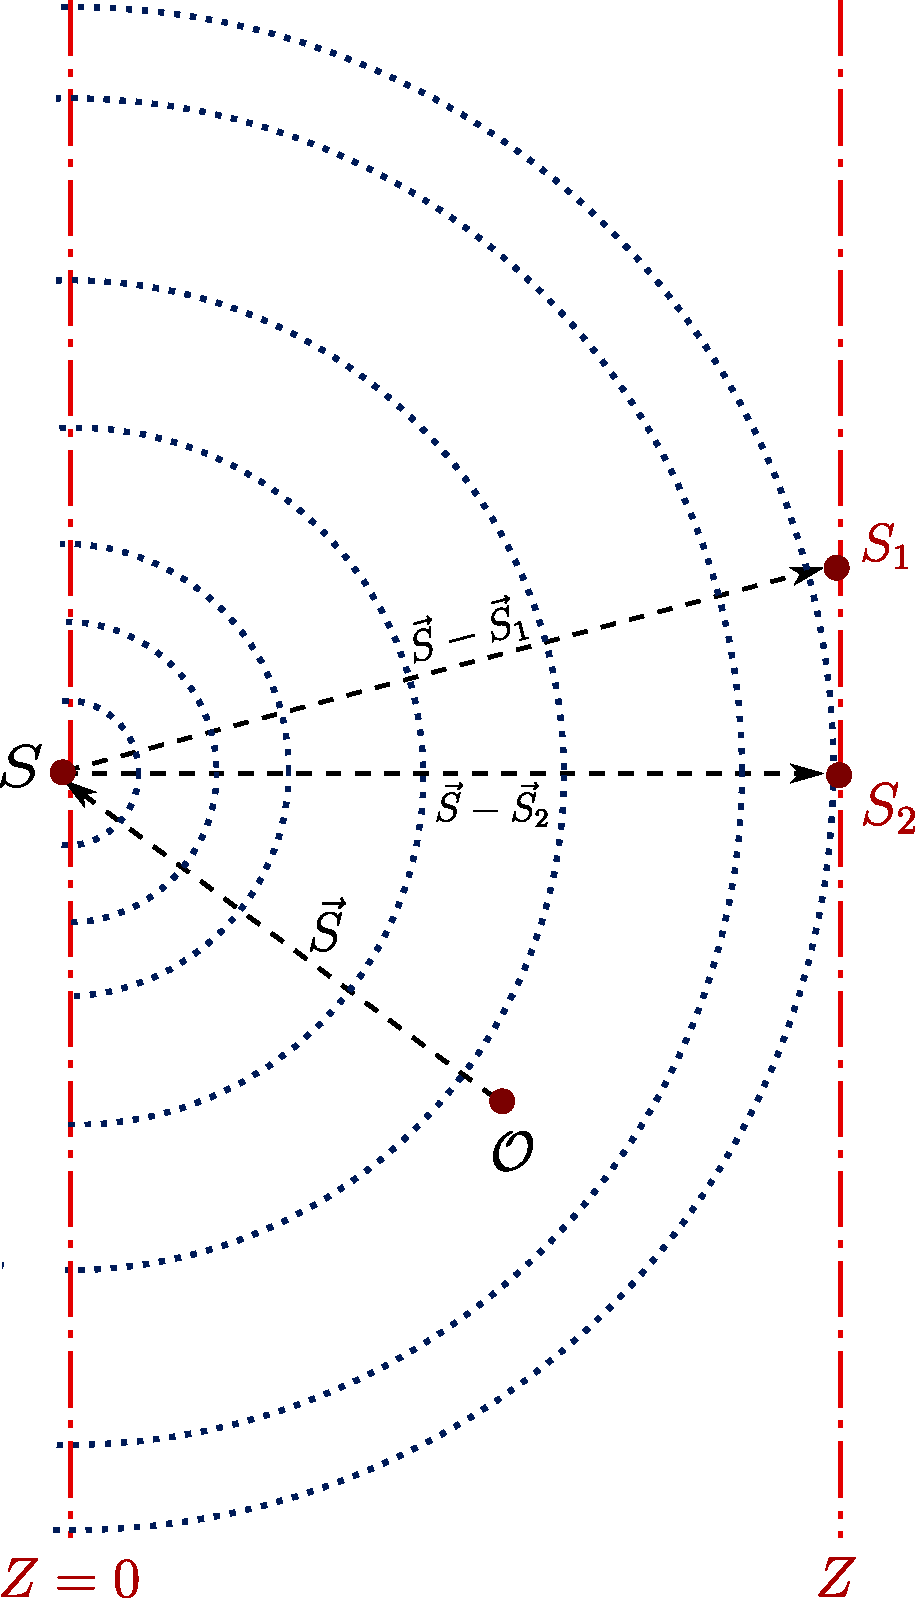
\includegraphics[width=0.65\linewidth]{Capitulo 2/Figuras/FourierGamma}
			\caption{La coherencia mutua propagada al campo lejano es la transformada de Fourier de la distribución de intensidad $\Gamma_0(\vec{S})$ de la fuente.}
			\label{fig:fouriergamma}
		\end{figure}

		¿Cómo podemos saber en qué dirección fluye el tiempo? Esto puede sonar como una pregunta bastante fuera de contexto para estos apuntes, pero si pudiéramos viajar a la época dorada de Boltzmann, encontraríamos un acalorado debate de la época sobre cómo la física estadística le da una dirección al tiempo, una \textit{flecha}. Parafraseando a Boltzmann, se dice que \textit{el tiempo avanza en la dirección en que las correlaciones aumentan}. Si observamos el teorema de van Cittert-Zernike, podemos partir de dos fuentes completamente no correlacionadas que, sin embargo, a medida que se propagan, van correlacionándose gradualmente; el tiempo crece y con él la coherencia, hasta llegar a un punto en el que la radiación de esas fuentes es coherente. Este es, sin duda, uno de los resultados más fuertes y hermosos que podemos encontrar en la física estadística.
